\documentclass[letterpaper,12pt,openright,notitlepage]{report}

\usepackage[T1]{fontenc}
\usepackage[utf8]{inputenc}
%\usepackage[brazil]{babel}
\usepackage{indentfirst}
\usepackage{graphicx}

\usepackage{fancyref}
\usepackage{textcomp}
\usepackage{amsmath}
\usepackage{amssymb}
\usepackage{braket}
\usepackage{xcolor}
\usepackage{array}
\usepackage{pdfpages}
\usepackage{tabularx}
\usepackage[ampersand]{easylist}
\usepackage{nomencl}
\makenomenclature
\usepackage{etoolbox}

%\usepackage{sectsty}
%\chapterfont{\color{blue}}
%\sectionfont{\color{cyan}}

\usepackage[bold]{hhtensor}
\usepackage{setspace}
\usepackage{epigraph}
\usepackage[colorlinks]{hyperref}

\usepackage[small]{caption}
\setlength{\captionmargin}{20pt}

\renewcommand*\thesection{\arabic{section}}
\setcounter{secnumdepth}{3}
\setcounter{tocdepth}{3}
\usepackage{booktabs}

\newcommand{\tab}{\hspace{1cm}}
\definecolor{lightblue}{rgb}{0.45,0.45,0.95}
\definecolor{darkblue}{rgb}{0.12,0.15,0.49}
\definecolor{NewBlue}{rgb}{0,0,0.4}
\definecolor{RoyalBlue}{rgb}{0,0,0.6}

% Hyperlink options
%\usepackage[letterpaper,linktocpage]{hyperref}
\hypersetup{colorlinks=true,       
	linkcolor= NewBlue,          % color of internal links
	citecolor=blue,        % color of links to bibliography
	urlcolor=black,
	bookmarksnumbered=true,
	pdffitwindow=true, 
	%bookmarks=true,
    pdftitle={Master Dissertation},
    pdfauthor={Jorge H. Soares}
    }    
    
\usepackage[a4paper,top=3.0cm,bottom=3.0cm,left=2.0cm,right=2.0cm,footskip=1.5cm]{geometry}

%\setlength{\oddsidemargin}{0pt}
%\setlength{\topmargin}{20pt}
%\setlength{\headheight}{15pt}
%\setlength{\headsep}{25pt}
%\setlength{\textheight}{609pt}
%\setlength{\textwidth}{455pt}
%\setlength{\marginparsep}{35pt}
%\setlength{\marginparwidth}{35pt}
%\setlength{\footskip}{30pt}
%\setlength{\hoffset}{0pt}
%\setlength{\voffset}{0pt}
%\setlength{\paperwidth}{597pt}
%\setlength{\paperheight}{845pt}

\usepackage{fancyhdr}
\lhead{\leftmark}
\rhead{\thepage}
\lfoot{}
\cfoot{}
\rfoot{}
\pagestyle{fancy}
\usepackage{calc}     
    
\newcommand{\diff}[2]{\dfrac{d #1}{d #2}} %derivada
\newcommand{\n}{\text{n}}
\newcommand{\ddiff}[2]{\dfrac{d^2 #1}{d^2 #2}} %derivada segunda
\newcommand{\pdiff}[2]{\dfrac{\partial #1}{\partial #2}} %derivada parcial
\newcommand{\pddiff}[2]{\dfrac{\partial^2 #1}{\partial^2 #2}} %segunda derivada parcial
\newcommand{\dvol}{dV} %elemento de volume
\newcommand{\dsurf}{dA} %elemento de superficie
\DeclareMathOperator{\sen}{sen}
\newcommand{\dg}{$^\text{o}$}
\newcommand{\regmark}{\textsuperscript{\textregistered}}   
\newcommand{\subref}[2]{\ref{#1}\textcolor{NewBlue}{#2}}


\definecolor{NewBlue}{rgb}{0,0,0.4}
\definecolor{RoyalBlue}{rgb}{0,0,0.6}

%\usepackage{secdot} 
\usepackage{sectsty}
\chapternumberfont{\color{NewBlue}\Huge} 
\chaptertitlefont{\color{NewBlue}\Huge}
\sectionfont{\color{NewBlue}\large}
\subsectionfont{\color{RoyalBlue}\large}
\subsubsectionfont{\color{RoyalBlue}\small}

\newcommand{\gom}{g_\text{OM}}
\newcommand{\ml}{Matlab\textsuperscript{\textregistered} }
\newcommand{\cm}{Comsol\textsuperscript{\textregistered} }
\newcommand{\llink}{LiveLink\textsuperscript{\textregistered} }
\renewcommand{\figurename}{Fig.}
\renewcommand{\thesection}{\thechapter.\arabic{section}}
\usepackage{xspace}
\newcommand{\etc} {etc.\xspace}
\newcommand{\eg} {e.\,g.\xspace}
\newcommand{\ie} {i.\,e.\xspace}
\newcommand{\regist}{\textsuperscript{\textregistered}}
\newcommand{\trdmrk}{\textsuperscript{\texttrademark}}
\newcommand{\sinn}{Si$_3$N$_4$\text{ }}
\newcommand{\sio}{SiO$_2$\text{ }}
\newcommand{\comsol}{COMSOL\regist}
\newcommand{\livelink}{LiveLink\regist}
\newcommand{\matlab}{MatLab\regist}
\newcommand{\susce}[1]{\chi^{( #1)}}
\DeclareMathOperator{\RE}{\text{Re}}
\DeclareMathOperator{\IM}{\text{Im}}

\providecommand{\boldsymbol}[1]{\mbox{\boldmath $#1$}}
\graphicspath{{figuras/}}

\numberwithin{equation}{chapter}
\numberwithin{figure}{chapter}



\begin{document}

\def\figurename{Fig.}
\def\tablename{Tab.}

\thispagestyle{empty}

%\begin{figure}[httb]
%\begin{center}
%\includegraphics[width=2cm]{logo_unicamp}
%\end{center}
%\end{figure}
\begin{flushleft}
	
\includegraphics[height=2.5cm]{unicamp.pdf}
\end{flushleft}

\begin{center}
\begin{doublespacing}
{\large UNIVERSIDADE ESTADUAL DE CAMPINAS}\\
\vspace{0.5cm}
{\large INSTITUTO DE FÍSICA GLEB WATAGHIN}\\
\end{doublespacing}
\end{center}

\vspace{3cm}
\begin{center}

\begin{center}
\textsc{\large Jorge Henrique Soares}
\end{center}
\vspace{3cm}

\begin{center}
\textsc{\Large Third harmonic generation in optical microcavities}
\end{center}

\vspace*{0.3cm}

\begin{center}
\textsc{\large Geração de terceiro harmonico em microcavidades ópticas}
\end{center}

\vfill
\begin{center}
\textsc{\large Campinas\\2019}
\end{center}
\newpage

\end{center}
\newpage
\thispagestyle{empty}

\vspace*{0.6cm}
\begin{center}
\textsc{\large Jorge Henrique Soares}
\end{center}


\vspace*{0.6cm}

\begin{center}
\textsc{\Large Third harmonic generation in optical microcavities}
\end{center}

\vspace*{0.3cm}

\begin{center}
\textsc{\large Geração de terceiro harmonico em microcavidades ópticas}
\end{center}

\vspace*{0.6cm}

\begin{flushright}
\begin{minipage}{8.0cm}
Dissertation presented to the Gleb Wataghin Institute of Physics of the University of Campinas in partial fulfillment of the requirements for the degree of Master of physics, in the area of applied physics.

\vspace*{0.3cm}

Dissertação apresentada ao Instituto de Física Gleb Wataghin da Universidade Estadual de Campinas como parte dos requisitos para a obtenção do título de Mestra em física, na área de física aplicada.

\end{minipage}
\end{flushright}

\vspace*{0.8cm}
\begin{flushleft}
	\hspace{0.3cm} \textsc{Supervisor/Orientador: Thiago Pedro Mayer Alegre}
	
	\hspace{0.3cm} \textsc{Co-supervisor/Coorientador: Gustavo Silva Wiederhecker}
\end{flushleft}

\vspace*{0.5cm}

\begin{minipage}{7cm}
\scriptsize \textsc{Este exemplar corresponde à versão final da tese defendida pelo aluno Jorge Henrique Soares e orientada pelo Prof. Dr. Thiago Pedro Mayer Alegre.}
%\\[4mm]
%\rule{7.0cm}{0.2mm} \hfill 
\end{minipage}

\vspace*{0.5cm}

\null \vfill
\begin{center}
\textsc{\large Campinas\\2019}
\end{center}






\newpage %Text should be exclude, page will be include as pdf generated by CPG
Ficha Catalografica
\thispagestyle{empty}
\newpage %Text should be exclude, page will be include as pdf generated by CPG
Carta de Aprovação
\thispagestyle{empty}
\newpage

\thispagestyle{empty}
\vspace*{15cm}
\begin{epigraphs}
	%\qitem{\textsc{``One is all, all is one.''}}{\textsc{``Fullmetal Alchemist'', manga by Himoru Arakawa.}}
	\item{\textsc{``Oblivion''}}
\end{epigraphs}

\onehalfspacing

\clearpage
\phantomsection
\addcontentsline{toc}{chapter}{Agradecimento}
\chapter*{Agradecimento}
\thispagestyle{empty}
Agradecimento
\clearpage
\phantomsection
\addcontentsline{toc}{chapter}{Resumo}
\chapter*{Resumo}
\thispagestyle{empty}

Resumo em portugues
\clearpage
\phantomsection
\addcontentsline{toc}{chapter}{Abstract}
\chapter*{Abstract}
\thispagestyle{empty}

Abstract in English

%\thispagestyle{empty}
\thispagestyle{empty}{
    \begin{singlespacing}
        \tableofcontents
    \end{singlespacing}
}
%\newpage
%\thispagestyle{empty}

\thispagestyle{empty}{
    \begin{singlespacing}
        \renewcommand\nomgroup[1]
{%
    \item[\bfseries
        \ifstrequal{#1}{B}{Chapter 2}{%
        \ifstrequal{#1}{C}{Chapter 3}{%
        \ifstrequal{#1}{D}{Chapter 4}{%
        \ifstrequal{#1}{E}{Chapter 5}{%
        \ifstrequal{#1}{F}{Chapter 6}{%
        \ifstrequal{#1}{G}{Chapter 7}{}
        }}}}
        }
    ]
}

%Chapter 2
\nomenclature[B 6]{$q$}{Eletric Charge}
\nomenclature[B 7]{$\vec{p}$}{Dipole Moment}

\nomenclature[B 9]{$\vec{x}$}{Electron Displacement from Rest Position}
\nomenclature[B]{$\vec{E}$}{Electric Field}
\nomenclature[B]{\vec{D}}{Displacement Vector}
\nomenclature[B 3]{$\mu_0$}{Vacuum Permeability}
\nomenclature[B 6]{$\chi^{(n)}$}{with $n>1$, Nonlinear Electric Susceptibility}
\nomenclature[B]{$\vec{P}$}{Electric Polarization}
\nomenclature[B 5]{$\chi^{(1)}$}{Linear Electric Susceptibility}
\nomenclature[B 2]{$\epsilon_0$}{Vacuum Permittivity}
\nomenclature[B 1]{$c$}{Speed of Light in Vacuum}
\nomenclature[B 10]{$A_\alpha$}{Complex Amplitude of the Electric Field}

%Chapter 3
\nomenclature[C 1]{\vec{e}}{Space Dependent Part of the Electric Field}
\nomenclature[C 2]{\vec{h}}{Space Dependent Part of the Magnetic Field}
\nomenclature[C 3]{$\kappa$}{Total Cavity Loss}
\nomenclature[C 4]{$\kappa^{(i)}$}{Intrinsic Cavity Loss}
\nomenclature[C 5]{$\kappa^{(e)}$}{Coupling Cavity Loss}
\nomenclature[c 6]{$\omega$}{Frequency of the Source}
\nomenclature[C 7]{$\Delta$}{Laser Detuning}
\nomenclature[C 8]{$\mathcal{F}$}{Finesse}
\nomenclature[c ]{$\beta$}{Vacuum Wavenumber of Light}

%chapter 5
\nomenclature[E 1]{$A_{ii}$}{Self Phase Modulation of the $i$th mode}
\nomenclature[E 2]{$A_{ij}$}{Cross Phase Modulation of the $i$th mode due to the $j$th mode}
\nomenclature[E 3]{$B_{ij}$}{Coupling Coefficient between $i$th and $j$th modes}
\nomenclature[E 4]{$\delta\omega$}{Phase Detuning}
        \printnomenclature
    \end{singlespacing}
}

%\newpage
%\setcounter{page}{1}
\chapter{Introdução}
Contextualização do projeto. Comentários sobre microcavidades, dispositivos ópticos, óptica não-linear
\chapter{Nonlinear Optics}
\label{chap:2_nonlin_pol}
The model for nonlinear optical effects, as third harmonic generation, is already well-known in literature~\cite{Boyd2003}. However, in this Chapter we will describe the model for Harmonic Generation in a bulk material. Also, we shall look for the propagation of two waves coupled due to optical nonlinearity. This concepts shall be very useful to understand the dynamic of the generation of third harmonic in optical cavities.  

\section{Optical Polarization}
\label{sec:Optical_nonlinear}
An important subject of optical science to describe the interaction between light and matter is the existence of dipole moment per unit volume, which is called polarization. In a dielectric medium the polarization occurs mainly due to induced dipoles.

\begin{figure}[h!]
    \centering
    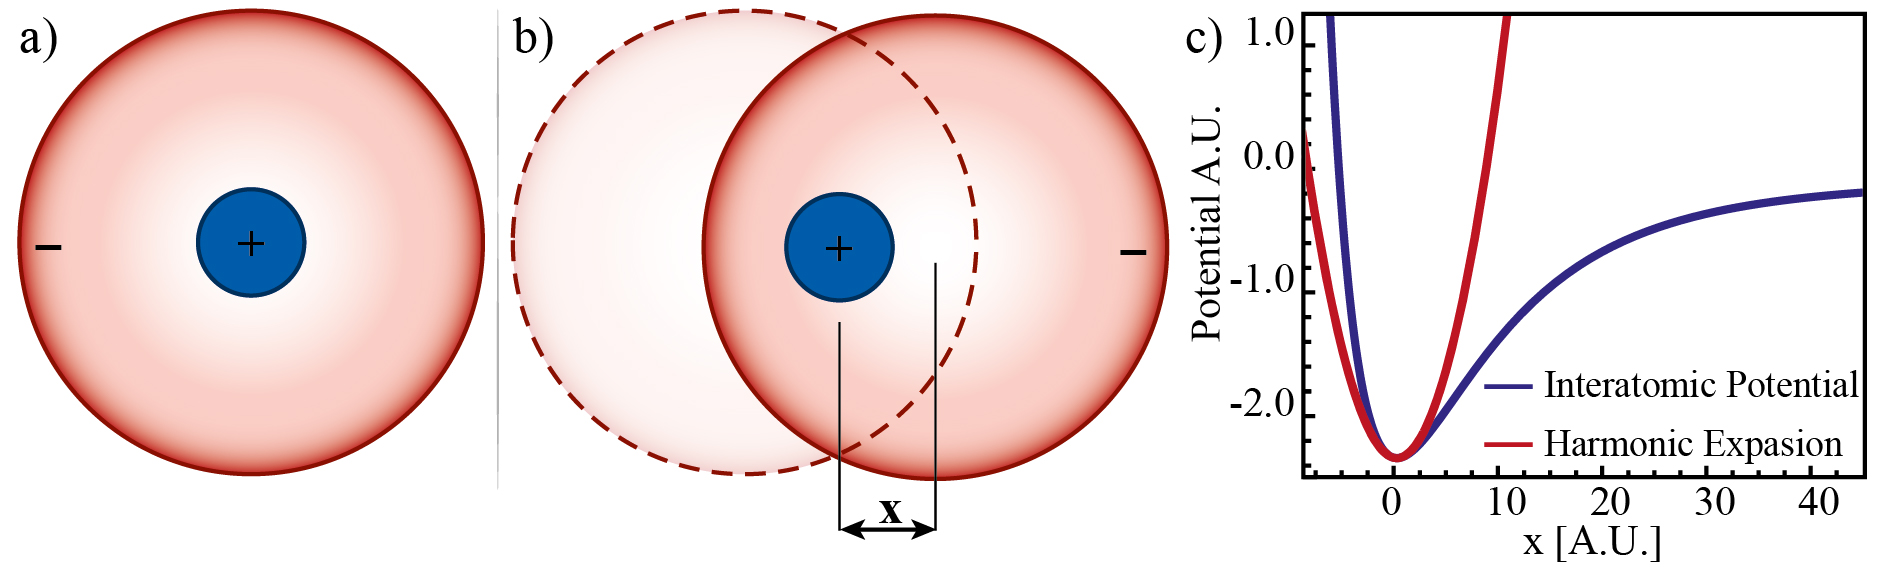
\includegraphics[width = 16cm]{figuras/Dissertation_atomic_polarization.jpg}
    \caption{\textbf{a) Atom in equilibrium:} the spherical symmetry of the atom makes it neutral for any external electric field. \textbf{b) Atom out of equilibrium:} If a strong enough external electric field are applied, it cause a displacement $x$ which generate a dipole with moment proportional on $x$. \textbf{c) Interatomic potential:} For a small displacement $x$ it is possible to approach the potential as an parable.}
    \label{fig:polarization}
\end{figure}
Lets consider a neutral atom placed in an external electric field $\vec{E}$. If the external electric field is negligible when compared with the internal electric field the initial equilibrium position is the concentric configuration, as shown in Fig.~\ref{fig:polarization}, this problem is analogous to the a solid spherical body charged with charge $q$ surrounded with a shell of charge $-q$. In a semiclasical approach we can consider all the charge concentrated in the center of each part~\cite{Griffiths2005}, which lead to a null total electric charge, hence to non electric field. However, the electron are free to move and thus the external electric field is able to displace the electron from the equilibrium position, creating a ionized dipole as shown in Fig.~\subref{fig:polarization}{b} (We consider that the external electric field isn't strong enough to deform the electronic cloud). It is easy to show that the dipole moment is proportional to displacement distance with the form~\cite{Griffiths2005}
\begin{equation}
    \vec{p} = q\vec{x}.
\end{equation}

When the external electric field is weak if compared with the interatomic electric field, we can approach the atomic potential to a parabolic, as show in Fig.~\ref{fig:polarization}c. The restoring force; therefore, is linear with distance. In such model, the polarization $\vec{p}$ is linear with the external electric field
\begin{equation}
    \vec{p} = \alpha \vec{E}.
\end{equation}
The constant $\alpha$ is called atomic polarization and depends on the atomic structure. This simple model is, in fact, in well agreement with experimental result.  

The result for a single atom can be easily extend for a solid body applying the principle of  superposition. In this way
\begin{equation}
    \vec{P} = \epsilon_0\chi^{(1)}\vec{E}.
\end{equation}
The information about the structure of the bulk material are contained in the constant $\susce{1}$; we call it linear electric susceptibility.

The assumption of weak external electric field implies in a small displacement, if compared with the atomic radius, otherwise we can't assume a parabolic potential due to the anharmonic form of the interatomic potential. 

In order to formulate a more general model, lets consider the motion of a electron in an anharmonic potential. Due to the spherical symmetry of the system, it is reasonable to assume that the motion of the electron occurs in the same direction on the applied electric field so we can avoid vectorial notation by define the generalized coordinate $x'$ in such way that the its real part is the displacement of the electron from the equilibrium position at this direction. We then have
\begin{equation}
    \ddot{x'} + 2\gamma\dot{x'} + \omega_0^2x'+ax'^2+bx'^3 = -eE(t)/m.
    \label{eq:motion_equation_electron}
\end{equation}
Here we assumed an applied time-dependent electric field given by $E(t)$, the electron charge as $-e$, a damping force of the form $-2m\gamma\dot{x'}$ and a restoring force given by
\begin{equation}
    F_\text{restoring} = -m\omega_0^2x' -max'^2 -mbx'^3, 
\end{equation}
where $a$ and $b$ are parameters that characterizes the strength of the nonlinearity. This restoring force corresponds to a potential energy with the form 
\begin{equation}
    U(x') = -\int F_\text{restoring} dx' = \frac{1}{2}m\omega_0^2x'^2 +\frac{1}{3}max'^3 +\frac{1}{4}mbx'^4.
\end{equation}

\begin{figure}[h!]
    \centering
    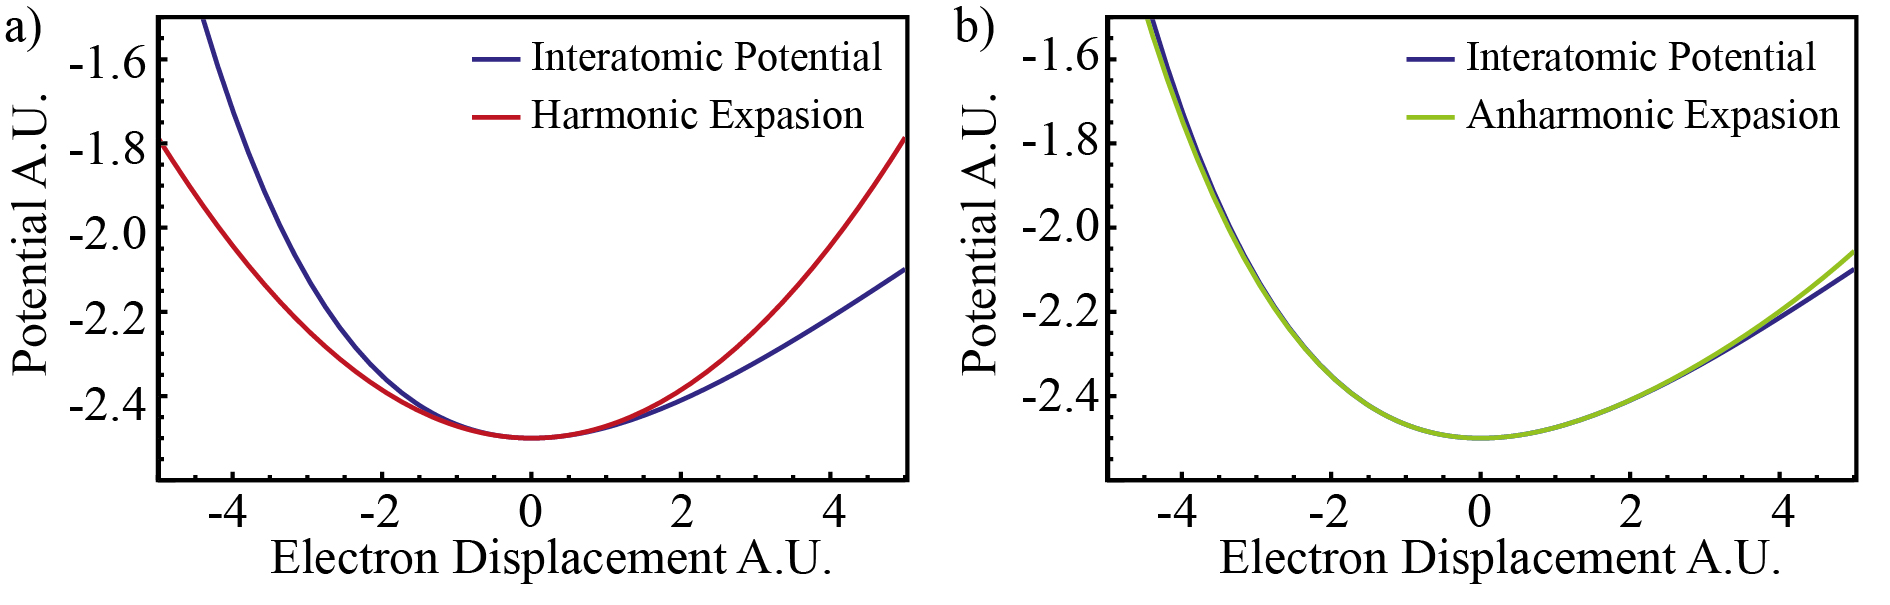
\includegraphics[width = 16cm]{figuras/Dissertation_interatomic_expassion.jpg}
    \caption{\textbf{a) Harmonic expansion:} The assumption of a parabolic potential are only valid if the Electron displacement are small when compared with the atom radius.\textbf{b) Anharmonic expansion:} Consider high order therms, anharmonic therms, for the expansion of the potential lead to a well agreement even when considered higher displacement.}
    \label{fig:expanssion}
\end{figure}
Eq.\ref{eq:motion_equation_electron} can be solved for using perturbation theory. Lets replace $E(t)$ by $\lambda E(t)$, %REWRITE: I must check Boyd calculus
\begin{equation}
    \ddot{x'} + 2\gamma\dot{x'} + \omega_0^2x'+ax'^2+bx'^3 = -\lambda eE(t)/m,
    \label{eq:pertubed_equation_electron}
\end{equation}
where $\lambda$ is continuous and ranges between zero and one. We seek for solutions in the form of power series of $\lambda$, that is 
\begin{equation}
    x' = \lambda x'^{(1)} + \lambda^2 x'^{(2)} + \lambda^3 x'^{(3)} +....
    \label{eq:x_pertubation_expanssion}
\end{equation}
This procedure give us a set of equations.
\begin{subequations}
    \begin{align}
        \ddot{x'}^{(1)} + 2\gamma\dot{x'}^{(1)} + \omega_0^2x'^{(1)} &= -eE(t)/m,\label{eq:first_order_pertubation}\\
        \ddot{x'}^{(2)} + 2\gamma\dot{x'}^{(2)} + \omega_0^2x'^{(2)}+a\left(x'^{(1)}\right)^2 &= 0,\label{eq:second_order_pertubation}\\
        \ddot{x'}^{(3)} + 2\gamma\dot{x'}^{(3)} + \omega_0^2x'^{(3)}+     2ax'^{(1)}x'^{(2)} +b\left(x'^{(1)}\right)^3 &= 0\label{eq:thirdt_order_pertubation}...    
    \end{align}
\end{subequations}

It is easy to see that the first order equation, Eq.~\ref{eq:first_order_pertubation}, is a problem of a forced harmonic oscillator. If considered a harmonic electric field with module $E(t) = Ee^{-i\omega t}$, for the steady-state we have
\begin{equation}
    x'^{(1)}(t) = \tilde{x}^{(1)}e^{-i\omega t}.
\end{equation}
The amplitude have the form
\begin{equation}
    \tilde{x}^{(1)} = -\frac{e}{m}\frac{E}{B(\omega)}.
\end{equation}
The function $B(\omega)$ are defined as $B(\omega) = \omega_0^2-\omega^2-2i\omega\gamma$.

Now we are able to rewrite Eq.~\ref{eq:second_order_pertubation} using the term in $x'^{(1)}$ as a driving force, which give us
\begin{equation}
    \ddot{x'}^{(2)} + 2\gamma\dot{x'}^{(2)} + \omega_0^2x'^{(2)} = a\left(\tilde{x}^{(1)}\right)^2e^{-i2\omega t}.
    \label{eq:second_order_motion_eq}
\end{equation}

Here we get a interesting result. Our system was initially drove by a harmonic force with frequency $\omega$, the anharmonicity of the interatomic potential bring forth a driven force with frequency $2\omega$. 

The steady-state solution of Eq.~\ref{eq:second_order_motion_eq} have the form
\begin{equation}
    x'^{(2)}(t) = \tilde{x}^{(2)}e^{-i2\omega t}.
\end{equation}
with the amplitude given by
\begin{equation}
    \tilde{x}^{(2)} = -\frac{a\left(eE\right)^2}{m^2B(\omega)^2B(2\omega)}.
\end{equation}

The same procedure for Eq.~\ref{eq:thirdt_order_pertubation} give us a perturbation with frequency $3\omega$, with the form 
\begin{equation}
    x'^{(3)}(t) = \tilde{x}^{(3)}e^{-i3\omega t},
\end{equation}
with amplitude
\begin{equation}
    \tilde{x}^{(3)} = -\frac{\left(eE\right)^3}{m^3B(\omega)^3B(3\omega)}\left(b+\frac{2a ^2}{B(2\omega)}\right).
\end{equation}

Eq.~\ref{eq:x_pertubation_expanssion} now give us a important insight. Even though the drive force due the external electric field is well defined with frequency $\omega$, the solution for the motion of the electron around the rest position gives us an harmonic series
\begin{equation}
    x'(t) = \lambda \tilde{x}^{(1)}e^{-i\omega t} + \lambda^2 \tilde{x}^{(2)}e^{-i2\omega t} + \lambda^3 \tilde{x}^{(3)}e^{-i3\omega t} +....
\end{equation}
Here we define the component drive by the external force as the fundamental mode of the motion of the electron and the high order terms are called second and third harmonic (later, we will apply this nomenclature for the optical mode).%REWRITE: I have defined nothing.  

This calculus can easily be extended to a vector analyse, along with the definition of dipole moment we can write
\begin{equation}
    \vec{p} = q\left(\lambda\vec{\tilde{x}}^{(1)}e^{-i\omega t}+\lambda^2\vec{\tilde{x}}^{(2)}e^{-i\omega t}+\lambda^3\vec{\tilde{x}}^{(3)}e^{-i\omega t}+... \right).
\end{equation}
For a bulk we have
\begin{equation}
    \vec{P} = \epsilon_0\chi^{(1)}\vec{E} + \epsilon_0\Bar{\chi}^{(2)}\vec{E}^2+\epsilon_0\Bar{\chi}^{(3)}\vec{E}^3+....
\label{eq:nonlim_pol}
\end{equation}
Note that the nonlinear susceptibility, $\Bar{\chi}^{(2)}$, $\Bar{\chi}^{(3)}$, are rank 2 and rank 4 tensors, respectively.

The main reason behind the math showed in this section is to make clear and intuitive that the generation of high orders harmonics occurs only due the interaction between an incident wave and the matter. This will be an important statement further below. 
%Now that I have convinced you that an anharmonic potential are able to generate high orders harmonic in the motion of the electrons leading to nonlinear terms for the polarization.% REWRITE.

\section{Wave Equation}
\label{sec:wave_equation}

We have looked on how the interaction between a harmonic wave electromagnetic wave and a nonlinear material generate high order harmonics. Lets now suppose the existence of two waves with different frequency and consider the effect of polarization upon the wave equation for a nonlinear optical medium~\cite{Boyd2003}. 

Starting with Maxwell's equations

\begin{subequations}
    \begin{alignat}{2}
        &\nabla\cdot\vec{D}  &&= 0,\\
        &\nabla\cdot\vec{B}  &&= 0,\\
        %\nabla\times\vec{E} &=  i \omega\vec{B}\\
        &\nabla\times\vec{E} &&= -\frac{\partial\vec{B}}{\partial t},\\ 
        %\nabla\times\vec{H} &= -i \omega\vec{D}\nabla\times\vec{E}
        &\nabla\times\vec{H} &&= \frac{\partial\vec{D}}{\partial t}.
    \end{alignat}
    \label{eq:max_eq}
\end{subequations}

We consider a nonmagnectic material, hence
\begin{equation}
    \vec{B} = \mu_0 \vec{H}
\end{equation}
%Otherwise, by consider a nonlinear medium, for the electric field we have
%\begin{equation}
%    \vec{D} = \epsilon_0\vec{E} + \vec{P}
%\end{equation}
%where $\vec{P}$ are given by Eq.~\ref{eq:nonlim_pol}.
%
In the absence of free charges and currents, we can then rewrite the Maxwell's equations in wave equation form for the electric field 
\begin{equation}
    \nabla^2\vec{E} - \frac{1}{\epsilon_0 c^2}\frac{\partial^2}{\partial t^2}\vec{D} = 0
\end{equation}
Finally, considering an nonmagnetic and nonlinear medium we can write the electric displacement field as
\begin{subequations}
    \begin{align}
        \vec{D} &= \epsilon_0\vec{E} +\vec{P},\\
        \vec{P} &= \vec{P}^{(1)} + \vec{P}^{(NL)}.
    \end{align}
\end{subequations}
In order to simplify the math, we split the polarization vector $\vec{P}$ in a linear part, given by $\vec{P}^{(1)} = \epsilon_0\chi^{(1)}\vec{E}$, and a nonlinear part $\vec{P}^{(NL)}$ given by all the remaining nonlinear terms of Eq.~\ref{eq:nonlim_pol}, so we have

\begin{equation}
    \nabla^2\vec{E} +\frac{\n^2}{c^2}\frac{\partial^2}{\partial t^2}\vec{E} = -\frac{1}{\epsilon_0 c^2} \frac{\partial^2}{\partial t^2}\vec{P}^{NL}.
    \label{eq:wave_equation_nonlinear}
\end{equation}
The refractive index, n, can be write as $\n^2= 1 + \chi^{(1)}$ and is a function of the frequency.

The following procedure can be applied for multiple nonlinear terms; however, since this is not the focus of this dissertation, we will proceed considering only the second order term. In such case

\begin{equation}
    \vec{P}^{NL} = \vec{P}^{(2)} = \epsilon_0\Bar{\chi}^{(2)}\vec{E}\vec{E}.
    \label{eq:nonlinear_polarization}
\end{equation}
%The total electric field is the sum of different frequency waves, for the second harmonic generation we have
Here, just for formality, was used explicitly the tensorial form of the nonlinear polarization and fields; however we will consider the case of a $z$ propagating wave in a isotropic medium, which enable us to use the nonlinear susceptibility as a scalar.

We are interested in the problem of how two different wave propagating in the same medium interact, wherefore the total electric field are the sum of this wave 
\begin{equation}
    \vec{E} = \vec{E}_1 + \vec{E}_2.
    \label{eq:total_field}
\end{equation}
The electric field of each wave can be write as    
\begin{equation}
    \vec{E}_\alpha = A_\alpha e^{i(k_\alpha z-\omega_\alpha t)}\hat{z} + c.c., \text{ for $\alpha = 1,2$}.
\end{equation}
As we saw in the Sec~\ref{sec:Optical_nonlinear}, the second order nonlinearity generate a wave with exactly twice the fundamental frequency, so $\omega_2 = 2\omega_1$. 

We are assuming that there is no other process beside second harmonic generation, resulting in a nonlinear polarization with two components, so that   
\begin{subequations}
    \begin{alignat}{1}
        \vec{P}^{(2)} &= \vec{P}^{(2)}_1+\vec{P}^{(2)}_2\\
        \vec{P}^{(2)}_\alpha &= P^{(2)}_\alpha e^{-i\omega_\alpha t}\hat{z}+c.c., \text{ for $\alpha$ = 1,2}.
    \end{alignat}
    \label{eq:nonlinear_polarization_harmonic_form}
\end{subequations}
%Due to the harmonic time dependence of the field, we can use $\frac{\partial}{\partial t} = -i\omega$, then Eq.~\ref{eq:wave_equation_nonlinear} can be write for each frequency, 

The left side of Eq.~\ref{eq:wave_equation_nonlinear} are composed by linear operators, we can write it as the sum of two equations. On the other hand, the left side of Eq.~\ref{eq:wave_equation_nonlinear} is, obviously, nonlinear which lead us to a system of two equation when arranging the therms with same harmonic the terms with the same time dependency  
\begin{subequations}
    \begin{alignat}{1}
        \frac{\partial^2}{\partial z^2}\vec{E}_1 +\frac{\omega_1^2}{c^2}\n_1^2 \vec{E}_1 = -\frac{\omega_1^2}{\epsilon_0 c^2} \vec{P}^{(2)}_1 \\
        \frac{\partial^2}{\partial z^2}\vec{E}_2 +\frac{\omega_2^2}{c^2}\n_2^2 \vec{E}_2 = -\frac{\omega_2^2}{\epsilon_0 c^2} \vec{P}^{(2)}_2
    \end{alignat}
\end{subequations}

Calculating Eq.~\ref{eq:nonlinear_polarization} and Eq.~\ref{eq:total_field}, comparing with Eq.~\ref{eq:nonlinear_polarization_harmonic_form} it is possible, and quit easy, to find that
\begin{subequations}
    \begin{align}
        P^{(2)}_1 &= 2\epsilon_0\chi^{(2)} A^*_1 A_2e^{i(k_2-k_1)z}\\
        P^{(2)}_2 &= \epsilon_0\chi^{(2)} {A_1}^2e^{i2k_1z}
    \end{align}
\end{subequations}


We can now analyze each frequency component, and simplify the equations by suppressing the vectorial notation. The full system of propagating wave equations are give by 
%\begin{subequations}
%    \begin{align}
%       \frac{\partial^2}{\partial z^2}A_1e^{ik_1z} +\frac{\omega_1^2}{c^2}\n_1^2 A_1e^{ik_1z} &= -2\frac{\omega_1^2 \chi^{(2)}}{\epsilon_0 c^2} A^*_1 A_2e^{-i\Delta kz}\\
%       \frac{\partial^2}{\partial z^2}A_2e^{ik_2z} +\frac{\omega_2^2}{c^2}\n_2^2 A_2e^{ik_2z} &= -\frac{\omega_2^2\chi^{(2)}}{\epsilon_0 c^2} A_1^2e^{i\Delta k z}
%    \end{align}
%\end{subequations}
\begin{subequations}
    \begin{align}
       \frac{\partial^2}{\partial z^2}A_1 +\frac{\omega_1^2}{c^2}\n_1^2 A_1 &= -2\frac{\omega_1^2 \chi^{(2)}}{c^2} A^*_1 A_2e^{-i\Delta kz}\\
       \frac{\partial^2}{\partial z^2}A_2 +\frac{\omega_2^2}{c^2}\n_2^2 A_2 &= -\frac{\omega_2^2\chi^{(2)}}{c^2} A_1^2e^{i\Delta k z}
    \end{align}
    \label{eq:coupled_wave_equation_SHC}
\end{subequations}
Here was defined the phase mismatch between the waves as
\begin{equation}
    \Delta k = 2k_1 - k_2.
\end{equation}

Eq.~\ref{eq:coupled_wave_equation_SHC} give us how the amplitude of the wave, especially the second harmonic, depends on the phase mismatch. 

Solution for coupled-wave equation have already been demonstrated; however, we are not interested in a analytic form for the amplitude, we ended up solving Eq.~\ref{eq:coupled_wave_equation_SHC} using numerical methods.

\begin{figure}[th!]
    \centering
    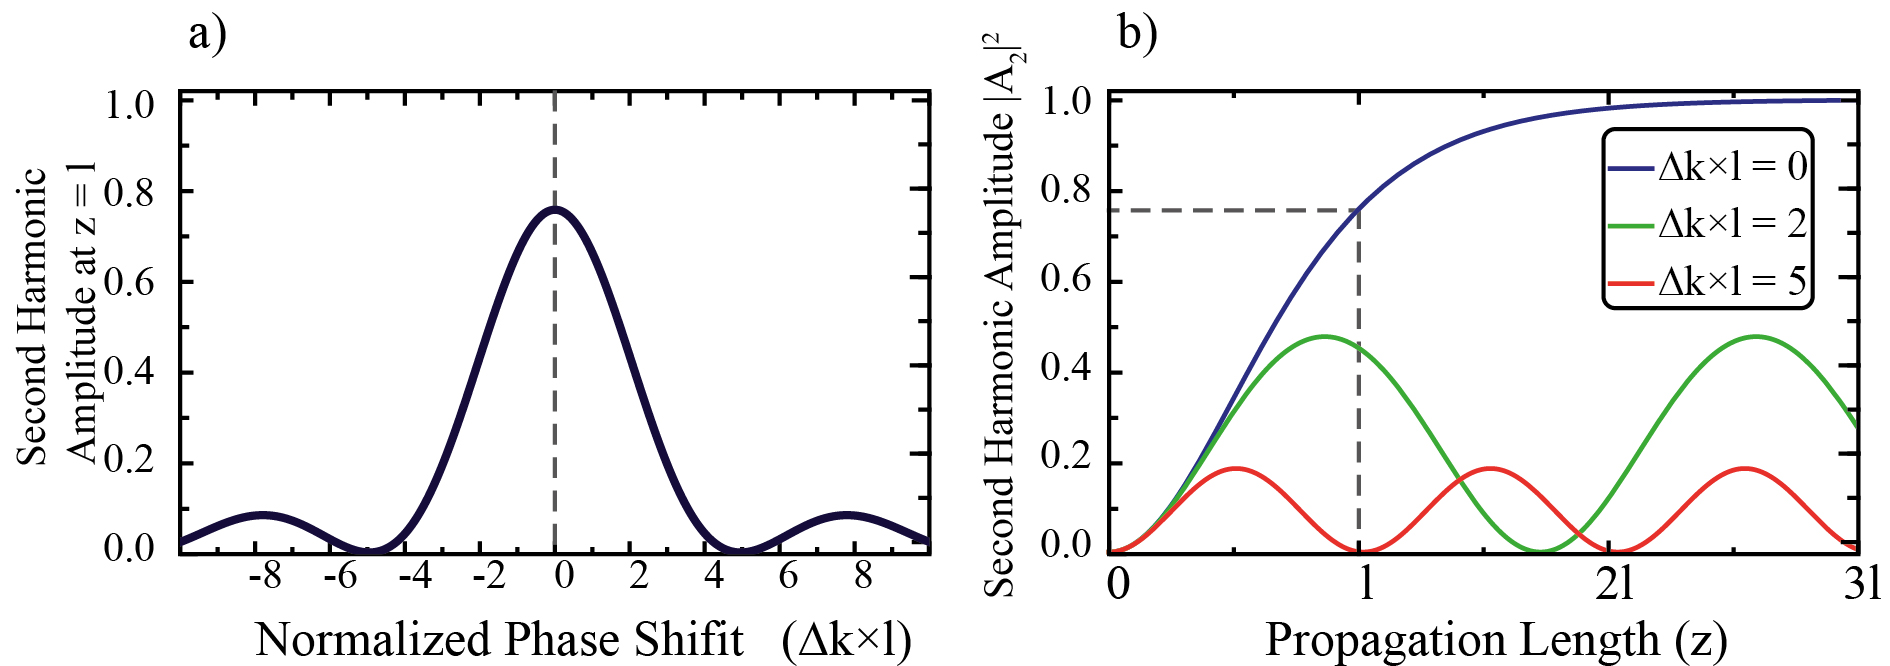
\includegraphics[width = 16cm]{figuras/Dissertation_coppled_eq_sol.jpg}
    \caption{\textbf{Coupled-wave equation numerical solution: a)} Modulus of the second harmonic amplitude, $|A_2|$, in function of $\Delta k \times l$ for $z = l$. \textbf{b)} Modulus of the second harmonic amplitude, $|A_2|$, in function of $z = l$ for different values of $\Delta k \times l$.}
    \label{fig:model_solution}
\end{figure}

In order to normalize the equations we define $l$ as the distance where, for $\Delta k = 0$, $75\%$ of the energy in the fundamental mode have been transferred for the second harmonic mode. 

Analysing the results presented in Fig.~\ref{fig:model_solution} it is possible observe two interesting, and indeed important, behaviors. Fig.~\subref{fig:model_solution}{a} shows that the amount of energy in the second harmonic model is maximum for $\Delta k = 0$; moreover, Fig.~\subref{fig:model_solution}{b} shows that the steady state are only reached for $\Delta k = 0$, any other value of $\Delta k$ lead to an oscillation as a function of the propagation distance.

\section{Conclusion}
Despite the focus of this project was not mathematically describe properties of material nor the propagation of coupled waves, we use this chapter to presents some quietly superficial math to reach two important conclusions.

First, we got from Sec~\ref{sec:Optical_nonlinear} that the wave generated due to second order nonlinearity presents exactly twice of the fundamental frequency, and this result come just from the interaction between the light and matter. 

Second, the Sec~\ref{sec:wave_equation} show us that an efficient conversion requires that the propagation of constant the second harmonic also to be double of the fundamental, otherwise we got a oscillatory dependence for the energy exchange and never reach a asymptote at the total conversion. 
% 
%
%However we got two, although obvious, important conclusion. First, was seen that the harmonic generation are result of the interaction between just the light and matter. Second, two modes are in phase matching only if both $\Delta \omega$ and $\Delta k$ are simultaneous zero.
%
Both conclusions will be better applied when we look for third harmonic generation in  modes confined in cavities. 

This result can be analogously make for third harmonic; however, it will give rinse for two additional terms responsible for a effect known as Kerr effect\cite{Barclay2005}. Due to third order nonlinearity the refractive index of the material change in amount proportional of the intensity of the electric field
\begin{equation}
    \text{n}(\omega_\alpha) = \text{n}_\alpha + \sum^{\beta=1,3} \text{n}_\beta |E_\beta|^2
    \label{eq:kerr_effect_free_wave}
\end{equation}

When considered, in typical laboratory condition, the Kerr effect includes a perturbation in the second term of the left side of Eq.~\ref{eq:wave_equation_nonlinear}. The following Chapter shall give us a more practical view of this effect.
\chapter{Optical Microcavity}
\label{chap:3_optical_cavity}

The last Chapter gave us two condition to optimize the Second Harmonic Generation, both are applicable for Third Harmonics\cite{Boyd2003}. It is desirable a long length of propagation, according with the Fig~\subref{fig:model_solution}{b}, and demand a large electric fields when compared with typical laboratory condition~\cite{Grubsky2005}. To compare, a silicon atom \footnote{We used a silicon atom as example just to simplify the atomic model, our cavities aren't build in silicon} has a atomic radius ($\rho_0$) of about $210$~pm and the atomic number of 14, with enable us to estimate   
\begin{equation}
   E_\text{atomic} = -\frac{1}{4 \pi \epsilon0}\frac{Z e^-}{\rho_0^2} %\approx 1.4\times10^{-9}\frac{Z}{\rho_0^2} 
    \approx 4.5\times10^{11}\text{V/m}.
\end{equation}

An approach to overpass this problem is using optical cavity. By recycle the photons trapped inside and confine them in a small space, the optical cavity enable to reach a large circulating power in a small effective area, which lead to high optical intensity and electric field. 

A typical optical mode, for a Whispering Gallery Mode (don't worry, it will be clear further) cavity with about $100~\mu$m of radius, presents a effective area ($A$) of around $10~\mu$m$^2$ and enable circulating power ($P$) as high as $1$~kW. We can estimate the electric field confined in a silicon cavity as 
\begin{equation}
    E_\text{confined} = \sqrt{\frac{2}{c\text{n}\epsilon_0}\frac{P}{A}} \approx 6 \times 10^7\text{V/m}.
\end{equation}

Where $\text{n}$ is the refraction index for silicon. Although it is order of magnitude lower than the interatomic electric field, the electric field confined in a optical cavity is high enough to observe nonlinear effects with input power much lower than required for non-resonate systems~\cite{Carmon2006,Farnesi2014,Chen-jinnai2012}. Moreover, the recycling of photons lead to a large optical path with small volume, enabling this kind of device efficient for integrated systems~\cite{Surya2018, Yang2018}.  

Therefore, it is important to understand the behavior of confined optical modes. Lets first introduce the theory for uncoupled mode for a arbitrary optical mode. Them we consider the nonlinearity of the medium to describe the coupled mode theory in the Chapter~\ref{chap:5_couple_mode}. 

\section{Single Mode Theory}
\label{sec:single_mode}

Considering a slowly varying envelop for the electromagnetic field, it is possible to write they as separable time and space function
\begin{equation}
    \genfrac{(}{)}{0 pt}{}{\vec{E}(\vec{r},t)}{\vec{H}(\vec{r},t)} = \sum_\alpha a_\alpha(t)\genfrac{(}{)}{0 pt}{}{\vec{e}_\alpha(\vec{r})}{\vec{h}_\alpha(\vec{r})}.
    \label{eq:general_mode}
\end{equation}
Each pair ($\vec{e_\alpha},\vec{h_\alpha}$) describe the spatial distribution of the $\alpha$th\footnote{$\alpha$ are a label and can assume any form, not necessary numerical} harmonic mode of frequency $\omega_\alpha$, hence 

\begin{equation}
    \nabla \times \genfrac{(}{)}{0 pt}{}{\vec{e}_\alpha(\vec{r})}{\vec{h}_\alpha(\vec{r})} = i\omega_\alpha \genfrac{(}{)}{0 pt}{}{\mu_0\vec{h}_\alpha(\vec{r})}{-\n^2\epsilon_0\vec{e}_\alpha(\vec{r})}.
    \label{eq:spatial_distribution}
\end{equation}

Applying the Eq~\ref{eq:general_mode} and Eq~\ref{eq:spatial_distribution} in the Maxwell's equations, Eq~\subref{eq:max_eq}{c} and Eq~\subref{eq:max_eq}{d}, we get

\begin{subequations}
    \begin{alignat}{2}
        &\sum_\alpha \left(\dot{a}_\alpha + i \omega_\alpha a\right) \mu_0 \vec{h}_\alpha &&= 0,\\
        &\sum_\alpha \left(\dot{a}_\alpha + i \omega_\alpha a\right) \text{n}^2\epsilon_0 \vec{e}_\alpha &&= -\frac{\partial}{\partial t}\vec{P}^{NL}.
    \end{alignat}
\end{subequations}

Calculating the expectation %, borrowing Dirac's notation, 
normalized by the energy stored in each mode, we them have 
\begin{equation}
    \dot{a}_\alpha + i \omega_\alpha a = -\frac{\braket{\vec{e}_\alpha|\partial_t\vec{P}^{NL}}}{2\epsilon_0\bra{\vec{e}_\alpha}\text{n}^2\ket{\vec{e}_\alpha}}.
    \label{eq:rate_equation_1}
\end{equation}
%(\bra{\vec{h}}\mu_0\ket{\vec{h}}+\bra{\vec{e}_\alpha}\epsilon_0\text{n}^2\ket{\vec{e}_\alpha})
%For solve the equations one must solve it therm by therm, which lead us to the rate equation for the amplitude of the $\alpha$th mode
%\begin{equation}
%    \dot{a}_\alpha + i \omega_\alpha a = 0.
%    \label{eq:rate_equation_1}
%\end{equation}
%wheres we normalized in suck way that $|a_\alpha|^2$ give the total energy stored in the $\alpha$th mode.

In order to compare our model with a real system, we shall introduce losses and source in Eq~\ref{eq:rate_equation_1}; We going to do both phenomenologically.

We will consider that the loss in energy is proportional to the stored energy inside the cavity. Moreover, a source can be included as a combination in current and charge densities in Maxwell's equations, which is analogous to include a polarization term, $\vec{P}_{in}$, to the total polarization. The time dependence of $\vec{P}_{in}$ has to do only with the source, being independent of the intracavity fields.

This step introduce some extra terms in the Eq~\ref{eq:rate_equation_1}, which results
\begin{equation}
    \dot{a}_\alpha = -\left(i\omega_\alpha +\frac{\kappa_\alpha}{2}\right)a_\alpha -\frac{\braket{\vec{e}_\alpha|\partial_t\vec{P}^{NL}}}{2\epsilon_0\bra{\vec{e}_\alpha}\text{n}^2\ket{\vec{e}_\alpha}}+\frac{\braket{\vec{e}_\alpha|\partial_t\vec{P}_{in}}}{\bra{\vec{e}_\alpha}\text{n}^2\ket{\vec{e}_\alpha}}.
\end{equation}
Wheres $\kappa_\alpha = \kappa^{(i)}_\alpha+\kappa^{(e)}_\alpha$ are the total rate of energy loss, composed by the intrinsic loss, suck material absorption and scattering loss, and couple loss due to coupling with the source. 

Finally, from input-output theory, it can be show that the feeding term can be written as $\sqrt{\kappa^{(e)}_\alpha}S_{in}(t)$, where $|S_{in}|^2$ gives the input power. Beside that, for our first analysis, we will consider that the nonlinear therm is small enough to be disregarded. This trick enable us to treat separately the temporal and spatial behavior of the optical modes. 

\subsection{Temporal Equations}

To describe the temporal evolution of the confined modes, we use the rate equation write as 
\begin{equation}
    \dot{a}_\alpha = -\left(i\omega_\alpha +\frac{\kappa_\alpha}{2}\right)a_\alpha +\sqrt{\kappa^{(e)}_\alpha}S_{in}(t).
    \label{eq:rate_equation2}
\end{equation} 

In typical laboratory condition, $S_{in}(t)$ correspond to a narrow spectral distribution centered at frequency $\omega$. We are able to rewrite Eq~\ref{eq:rate_equation2} in a rotating reference frame that turns the source terms into a constant by interchange $a_\alpha \rightarrow a_\alpha e^{-i\omega t}$
\begin{equation}
    \dot{a}_\alpha = -\left(i\Delta_\alpha +\frac{\kappa_\alpha}{2}\right)a_\alpha +\sqrt{\kappa^{(e)}_\alpha}S_{in}.
    \label{eq:rate_equation_unperturbed}
\end{equation}
where $\Delta_\alpha = \omega_\alpha - \omega$ is the detuning between the laser source and the cavity resonance frequency.
\begin{figure}[t!]
    \centering
    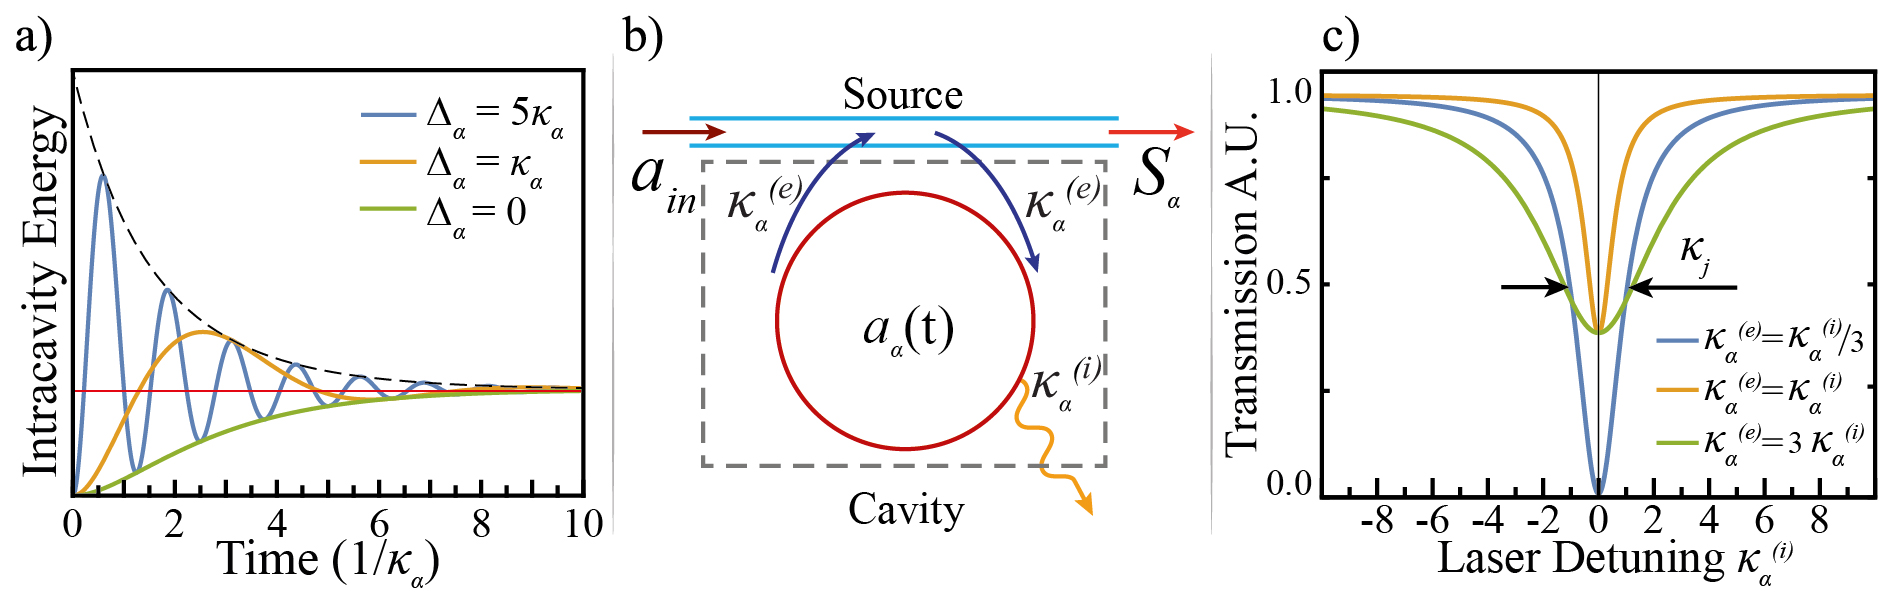
\includegraphics[width = 16cm]{Dissertation_rate_equation.jpg}
    \caption{\textbf{a) Time Dependence Solution of Intracavity Energy:} The energy stored in a cavity oscillate in a frequency $\Delta_\alpha$ and decay with a rate $\kappa_\alpha$ to the Stead Solution. \textbf{b) Lumped Mode:} Our System are compound by a cavity with a single mode $a_\alpha$ that presents intrinsic loss $\kappa_\alpha^{(i)}$. The mode couple with a Source at a rate $\kappa_\alpha^{(e)}$ and interacts with an incoming wave with complex amplitude $S_{in}$. The squared modulus of the output $S_\alpha$ are measured. \textbf{c) Spectroscopy of the $\alpha$th mode:} The transmission of the cavity gives a Lorentzian curve wheres the full width at half maximum correspond to the total loss. This graphic show it for three different regimes.}
    \label{fig:rate_equations_single_mode}
\end{figure}

Eq~\ref{eq:rate_equation_unperturbed} accepts harmonic solutions with frequency $\Delta_\alpha$. Nevertheless these solutions decay, with a  $\kappa_\alpha/2$ rate, into a steady state solution. We usually operates the system in a time scale much larger than $\kappa^{-1}$, thus we consider just the steady state solution, as show in Fig~\subref{fig:rate_equations_single_mode}{a}

We have already introduced the required formalism to describe our problem, at this point a more pictorial view of it would be very useful. For that we shall use the Fig~\subref{fig:rate_equations_single_mode}{b}. Lets consider our system composed by a optical cavity and a source. This cavity have a optical mode with amplitude $a_\alpha$, and present intrinsic energy loss $\kappa_\alpha^{(i)}$ due scattering and absorption. The source carry a input wave $S_{in}$ at frequency $\omega$ which couple with the cavity at a $\kappa_\alpha^{(e)}$ rate, the optical mode coupling back with the source at the same frequency, in such way that this couple is seen as a loss channel by the cavity. The outgoing wave, defined as $S_\alpha$, carry information about the source and the optical mode, in this way
\begin{equation}
    S_\alpha = S_{in} - \sqrt{2 \kappa_\alpha^{(e)}}a_\alpha.
\end{equation}
For the steady state solution we have $\dot{a} = 0$, which lead us to define the transmission of the cavity as
\begin{equation}
    T = \left|\frac{S_\alpha}{S_{in}}\right|^2 = \frac{\left(\kappa_\alpha^{(i)} -\kappa_\alpha^{(e)}\right)^2 + (2\Delta_\alpha)^2}{\left(\kappa_\alpha^{(i)} +\kappa_\alpha^{(e)}\right)^2 + (2\Delta_\alpha)^2}.
    \label{eq:single_mode_transmission}
\end{equation}

Typically, the experiment are made by sweep the source frequency, hence the detuning. The ration between the intrinsic loss and the coupling loss define the regime of the system; under coupled, for $\kappa_\alpha^{(e)} < \kappa_\alpha^{(i)}$, critical coupled, for $\kappa_\alpha^{(e)} = \kappa_\alpha^{(i)}$, and over coupled, for $\kappa_\alpha^{(e)} > \kappa_\alpha^{(i)}$; a comparison between each regime can be seen in the Fig~\subref{fig:rate_equations_single_mode}{c} 

As the capacity of recycle photons inside the optical cavity is a important feature, we should use a value to determine how efficiently our cavity does it. For this purpose we define the Finesse as the ratio between the mean lifetime of the photon inside the cavity and the round trip time, or in function of measurable parameters 
\begin{equation}
    \mathcal{F} = \frac{\text{Mean Lifetime}}{\text{Round Trip Time}} = \frac{FSR_\alpha}{\kappa_\alpha}.
    \label{eq:finesse}
\end{equation}
Where $FSR_\alpha$ is the Free Spectral Range of the $\alpha$th mode. Then the intracavity power is equal the input power time $\mathcal{F}$.

However, for our system the round trip time and the mean lifetime are coupled, in the sense that we aren't able to increase or decrease the round trip time without affect the mean lifetime, hence we define the Quality factor ($Q$) as the ration between the resonance frequency of the mode ($\omega_\alpha$) and the bandwidth ($\kappa_\alpha$) to determine the efficiency of our cavity to store photons, supposing that the $FSR_\alpha$ are nearly the same. 

In order to better understand the concept of Free Spectral Range and how do it lead us to the round trip time we must develop the spatial treatment of the modes. 
\subsection{Spatial Equations}

Initially lets consider a propagating wave at frequency $\omega$. From the Maxwell's equations it is possible to write
\begin{subequations}
    \begin{alignat}{2}
    &\nabla^2\vec{h}_\alpha+\beta^2n^2\vec{h}_\alpha &&= \nabla(\nabla\cdot\vec{h}_\alpha),\\
    &\nabla^2\vec{e}_\alpha+\beta^2n^2\vec{e}_\alpha &&= \nabla(\nabla\cdot\vec{e}_\alpha).
    \end{alignat}
    \label{eq:wave_eq_full}
\end{subequations}
Here we defined $\beta = \omega/c$, where $c$ is the speed of light in the vacuum. As the medium that we are interested presents uniform refraction index, we can solve Eq~\ref{eq:wave_eq_full} separately for the region inner and outer of the cavity, them match the boundaries conditions, in such case the right side of the equation are null for each region. 

We shall assume that the solution is a wave that propagate in $z$ direction with the form $e^{ik_\alpha z}$, hence the Eq~\ref{eq:wave_eq_full} can be rewrite as 

\begin{subequations}
    \begin{alignat}{2}
    &\nabla_t^2\vec{h}_\alpha+(\beta^2n^2-k_\alpha^2)\vec{h}_\alpha &&=0,\\
    &\nabla_t^2\vec{e}_\alpha+(\beta^2n^2-k_\alpha^2)\vec{e}_\alpha &&=0.
    \end{alignat}
    \label{eq:wave_eq}
\end{subequations}
Where $\nabla_t^2 = \nabla^2 - \partial^2/\partial z^2$.

\begin{figure}[b!]
    \centering
    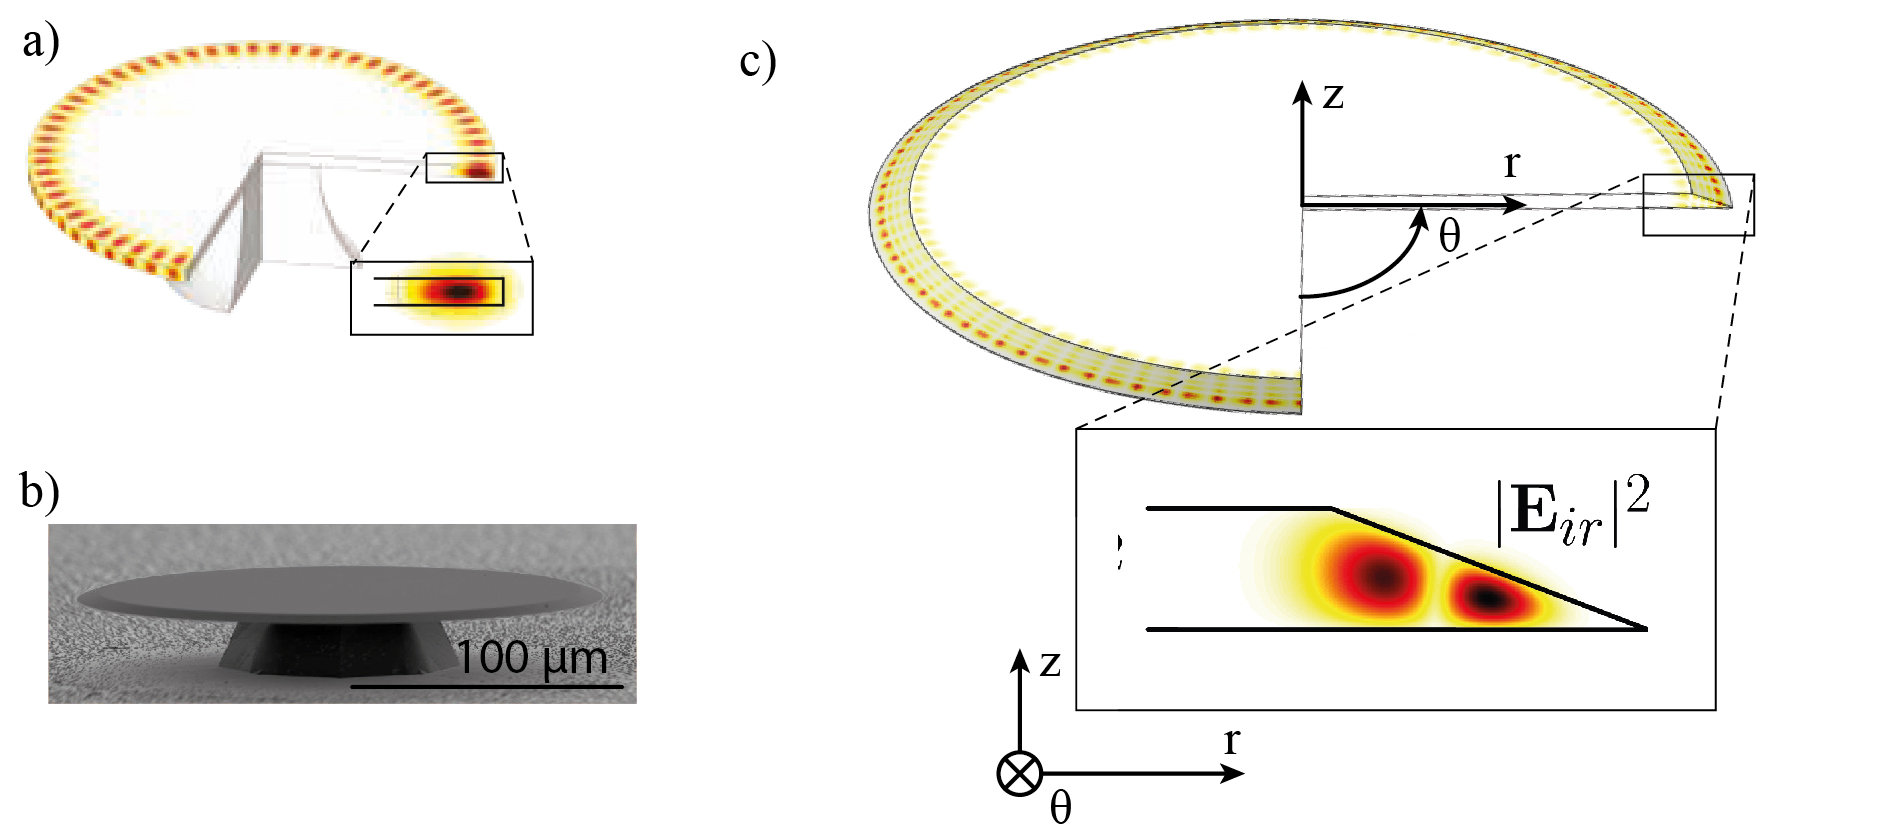
\includegraphics[width =16cm]{Dissertation_wgm.jpg}
    \caption{\textbf{a) Whispering Gallery Mode:} Intensity of the electric field confined in a disc cavity with about 10~$\mu$m radius. The WGM confine the optical mode in the edges of the cavity. \textbf{b) Wedge Cavity:} Image take from a Scanning Electron Microscope of the cavity used in this study. \textbf{c) Coordinates:} The coordinates of the problem are defined as that. This mode is a TM21 with $m = 526$ and frequency $\omega_\alpha/2\pi = 193.5$~THz}.
    \label{fig:wgm}
\end{figure}
It might be have been overlooked, but the Eq~\ref{eq:wave_eq} is a system with 6 equation; one for which field in each coordinate. The solution for this set of equation with boundary condition define the optical modes of our problem. To solve this equations we must apply consideration about symmetry; however we use numerical methods to solve it. We will use the commercial software COMSOL\regmark.
%, in Appendix~\ref{app:Comsol_Solution} we explained step by step how this solutions are done. 

Until now we have talk about generic electromagnetic modes, with no spatial boundary condition, in order to define them we must define the geometry of our cavity. Our device are based in disk microcavities, as show in Fig~\subref{fig:wgm}{a}, this kind of resonator presents the so called Whispering Gallery Modes (WGM), due to cylindrical symmetry. In order to archive high life time of the photons inside the cavity we use a wedge cavity. Fig~\subref{fig:wgm}{b} show a photo take using a Scanning Electron Microscope (SEM) of the cavity used in this study, the angle present at edge makes the electric field to be more parallel to the surface leading to lower loss due to scattering\cite{Lee2012}. The fabrication process have a important role in here, as we shall see below in Chapter~\ref{chap:4_fabrication}. 

The boundary condition lead to the characteristic equation in the form 
\begin{equation}
    F(k_r,k_\theta,k_z,\omega) = 0.
    \label{eq:char_eq}
\end{equation}
The solution of this equation as a function of the frequency $\omega$ give us the dispersion. 

The set of constants, $k_r,k_\theta,k_z$, that solve this equation define a mode. This constants can assume any complex value, which would hamper the nomenclature of the modes; fortunately, due to the confinement of the mode, we can correlate this constants with a integer number. The WGM are labeled in the format TExy and TMxy modes, where x and y are integers correlated with $k_r$ and $k_z$, respectively. Beside that, given a TExy (TMxy) mode it can have several values of $m$, which is a integer correlated with $k_\theta$, it also define the family of the mode. The value of x,y and $m$ can be interpreted as the number of antinodes in the intensity of the electric field in each coordinate as defined in the Fig~\subref{fig:wgm}{c}. To clarify the nomenclature adopted in this dissertation, henceforward the term '$\alpha$th mode' are applied for a TExy or TMxy mode with any value of $m$. 

The solution of the Eq~\ref{eq:char_eq} give rise to the dispersion of the cavity. As the Round Trip Time depend on the group velocity, it can be extracted from the dispersion by the relation
\begin{equation}
    \text{Round Trip Time} \approx \frac{2\pi R}{v_g} = \frac{2\pi R}{d\omega/dk_\theta} 
\end{equation}

Due to the discretization of the values of $k_\theta$ we can be approached as a differentiation, leading to
\begin{equation}
    \frac{d\omega}{dk_\theta} \approx \frac{\Delta \omega}{\Delta k_\theta} = R\frac{\Delta \omega}{\Delta m}
\end{equation}
The $FSR$ is the linear frequency between two consecutive modes, so
\begin{equation}
    v_g \approx 2\pi R~FSR \Rightarrow \text{Round Trip Time} \approx FSR^{-1} 
\end{equation}

Now we have enough knowledge to understand how to experimentally characterize our devices. The following Section will treat this subject. 

\section{Optical Characterization}
\label{sec:optical_char}

The main relevant parameters to characterize an optical mode are the losses and the resonance frequency, which is done be measuring the transmission and compare with the Eq~\ref{eq:single_mode_transmission} from the single mode model. 

The experiment is made using the setup showed in the  Fig~\ref{fig:exp_mode_charac}a; A laser with tunable frequency are applied as source, a piezo tunes the size of the external cavity leading to a few GHz of modulation. A small part of the output light are directed to a frequency calibrator compound of a Mach Zehnder interferometer and a wavelength reference Hydrogen Cyanide (HCN) cell. An attenuator controls the input power in the cavity. The polarization of the input wave are controlled using a manual fiber polarization control. We use a tapered optical fiber to couple the source with the cavity. The transmission are measured using a power meter and the data are acquired using a DAQ. 
\begin{figure}[h!]
    \centering
    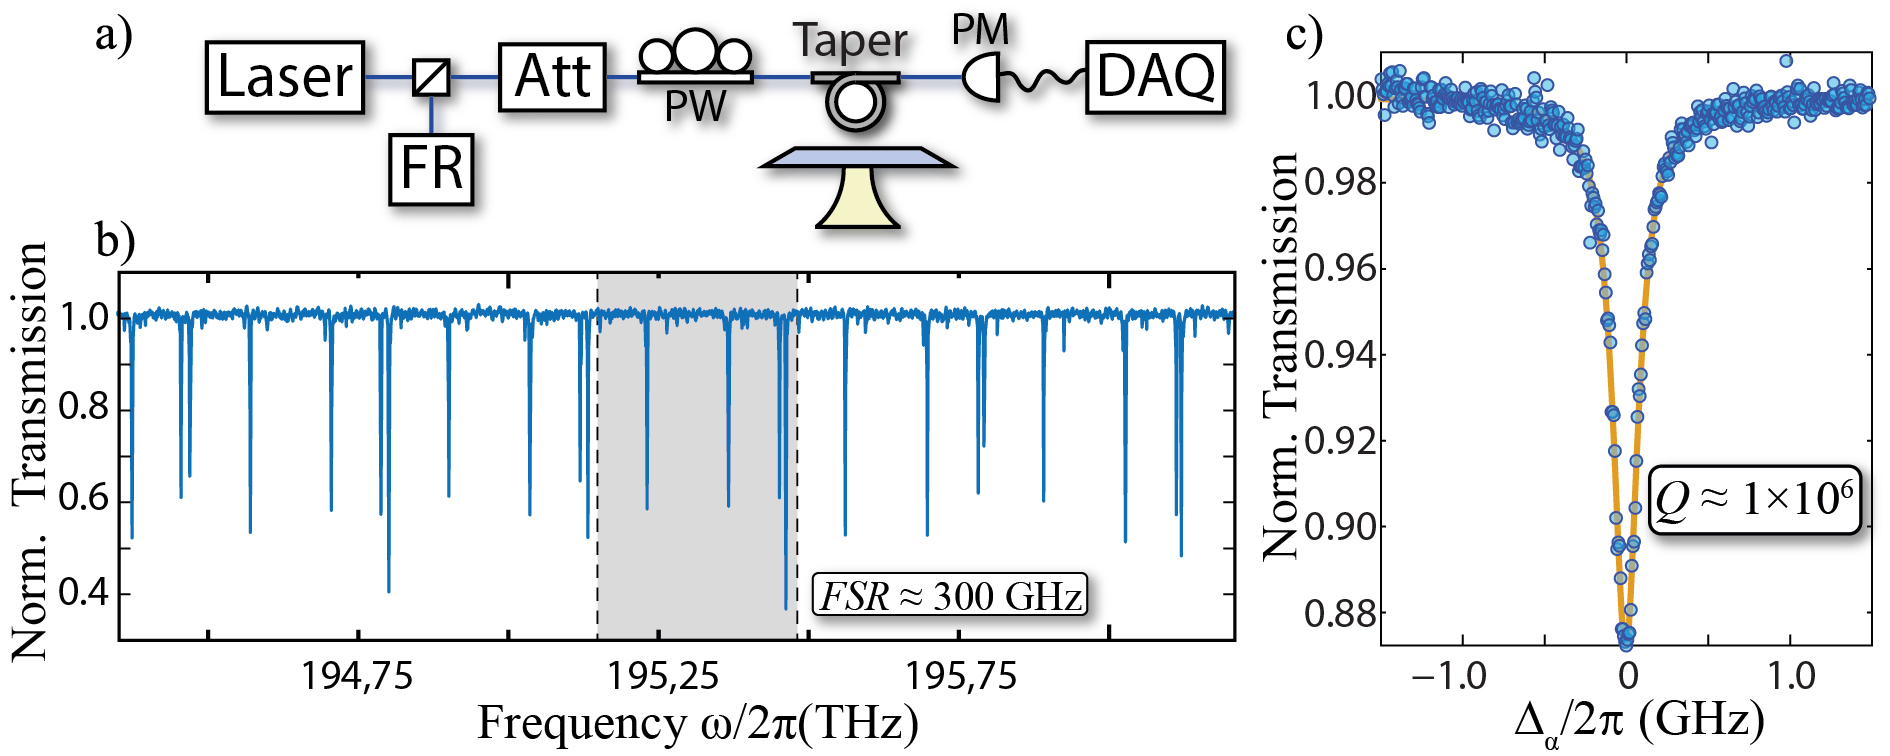
\includegraphics[width = 16cm]{figuras/Dissertation_optical_char_exp.jpg}
    \caption{\textbf{a) Experimental Setup:} The key components of the Setup is the Laser used as source, a tapered optical fiber that couple the source with the cavity and power meter to monitor the output. The frequency of the laser are precisely determined using a Frequency Reference (FR) composed of a Mach Zehnder interferometer and a Hydrogen Cyanide cell. We use a tunable attenuator (ATT) to control the input power. The polarization of the input wave is controlled using a fiber polarization control (PW). \textbf{b) Single Mode:} Transmission for a single mode used to measure the losses of the mode. \textbf{c) Broad Band Transmission:} spectroscopy of the cavity for a broad band to measured the Free Spectral Range.} 
    \label{fig:exp_mode_charac}
\end{figure}

The result, for a single mode, are presented in Fig~\ref{fig:exp_mode_charac}c). We use the Eq~\ref{eq:single_mode_transmission} to fit the data giving the values of $300$ MHz and $50$ MHz for the $\kappa_\alpha^{(i)}$ and $\kappa_\alpha^{(e)}$, respectively. The mode are at frequency $\omega_\alpha = 2\pi\times195.25$ THz which give us a $Q \approx 3\times10^6$.

Using an stepper motor instead of the piezo it possible to modulate the frequency in few THz enabling us to measure different families of modes, as show in Fig~\ref{fig:exp_mode_charac}c). The spectral distance of a mode in consecutive families give the $FSR_\alpha$ for the $\alpha$ mode. Our cavities present an FSR around $300$ GHz, which have to due mostly with the radius of the device. 

According to Eq.~\ref{eq:finesse}, we reached a finesse of about $\mathcal{F} \approx 1000$. A device with this parameters enable to amplify the incoming power, due to photons recycling, about $1000$ times. If a input power of $1$~W is used, a total of 1 kW circulating power is reached as mentioned before. In general terms, it make our device a good platform to generate nonlinear effects. 
%A Fraction of the losses are due the material absorption, when we are working with high intracavity power this absorption lead to a thermal effects called bistability. 


\section{Pump Bistability}
\label{sec:bistability}

The resonance frequency of the cavity are correlated with the refractive index of the material, which is a function of the temperature. Treating this as a perturbation problem, we can write 

\begin{subequations}
    \begin{alignat}{2}
        \frac{\Delta\omega_\alpha}{\omega_\alpha} &= -\frac{\Delta \text{n}_\text{eff}}{\text{n}_\text{eff}}\\
        \frac{\Delta\omega_\alpha}{\omega_\alpha} &= -\frac{\int \text{n}^2\vec{e}^*\Delta\text{n}(T)~\vec{e} d^3r}
        {\int \text{n}^2 |\vec{e}|^2 d^3r}
        \label{eq:termooptc_change}
    \end{alignat}
\end{subequations}
$T$ is the temperature of the optical mode. In a good approximation, considering a small variation in the temperature, we can write
\begin{equation}
    \Delta \text{n}(T) = \frac{d\text{n}}{dT}\Delta T
\end{equation}
Here, the $\Delta T$ is proportional from the amount of energy absorbed by the material. As we are interested just in the contribution of this effect not in a explicit formula we can suppress all the process of energy conversion in a single constant and write the variation in the frequency in function of the energy storage in the cavity, in such way
\begin{equation}
\frac{\Delta \omega_\alpha}{\omega_\alpha} = A |a_\alpha|^2
\label{eq:pertubation_bistaliti_cavity}
\end{equation}   

Including the contribution in the rate equation Eq~\ref{eq:rate_equation2} after the transformation of reference frame, the bistable rate equation can be write as 
\begin{equation}
\dot{a}_\alpha = -\left(i\Delta_\alpha + i\omega_\alpha A|a_\alpha|^2 + \frac{\kappa_\alpha}{2}\right)a_\alpha + \sqrt{\kappa^{(e)}_\alpha}S_{in}
\label{eq:rate_equation_bistable}
\end{equation}
The new term $A$ receives the name of self phase modulation (SFM), it represents how much the intensity of the optical mode affects the resonance frequency.

As usual, we looking to the steady state solution. Depending on the $\Delta$ value, this equation can present three different solutions. To visualize it, lets write the Eq~\ref{eq:rate_equation_bistable} as 
\begin{equation}
    |a_\alpha|^2 = \frac{4\kappa^{(e)}_\alpha |S_{in}|^2}{4\left(\Delta_\alpha + \omega_\alpha A|a_\alpha|^2\right)^2+\kappa_\alpha^2} 
\end{equation}

The Fig~\subref{fig:bistable}{a}
shows the plot of the LHS and RHS in function of $|a_\alpha|^2$. Depending on the value of $\Delta_\alpha$ and $|S_{in}|$ there are three different solutions for this equation, but the intermediate one is always unstable, which lead to the well-know bistable transmission show in Fig~\subref{fig:bistable}{b}
Controlling the input power using the attenuator, as showed in the setup of the Fig~\subref{fig:exp_mode_charac}{c}, it is possible to experimental measure the bistability, this measure are show in Fig~\subref{fig:bistable}{c}. We found a value of around $A\approx 5.7\times10^7$~J$^{-1}$.

As the pump frequency get closer to the resonance frequency, the intracavity power increases, which shifts the resonance to the red through self-phase modulation, until the pump frequency, $\omega$, reaches the resonance frequency, $\omega_\alpha$; at this point, the effective detuning is zero and the energy stored in the cavity it's maximum.  

\begin{figure}[t]
    \centering
    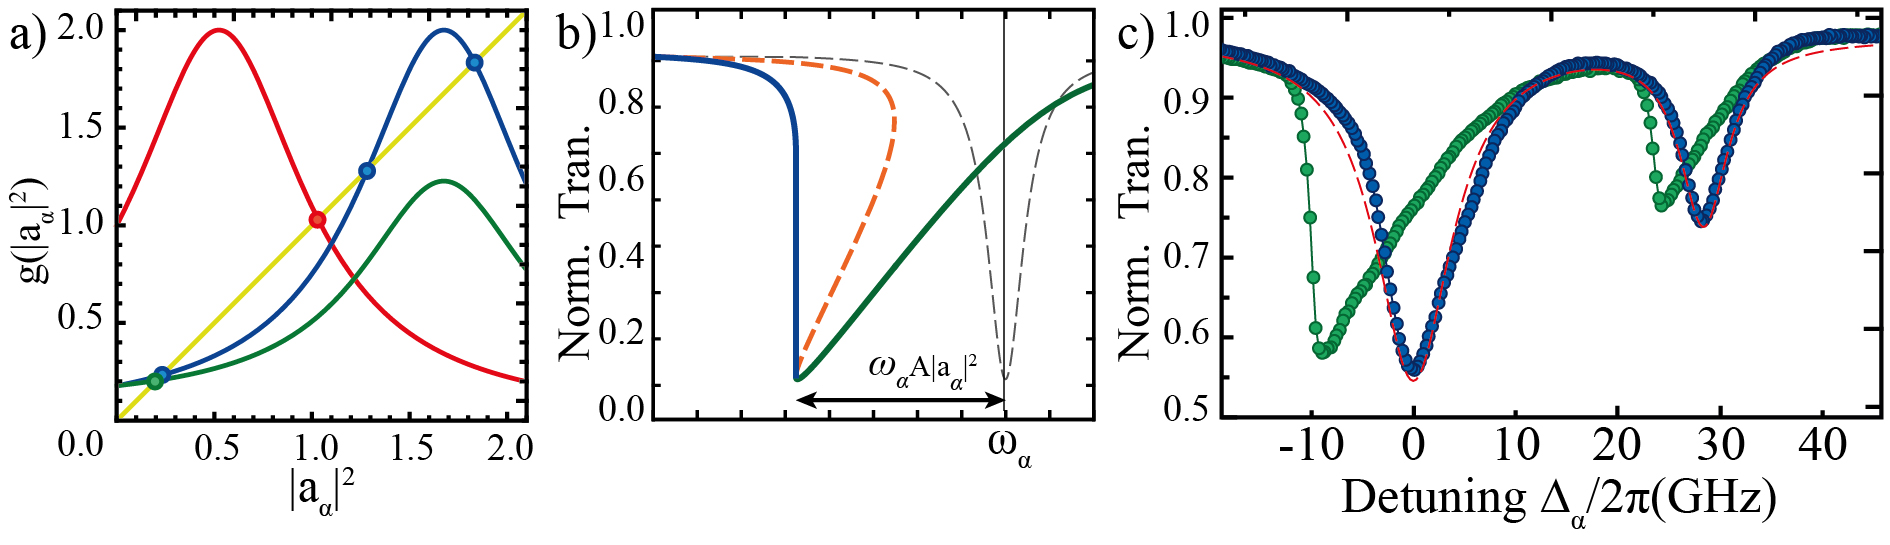
\includegraphics[width = 16cm]{Dissertation_bistabilite.jpg}
    \caption{\textbf{a) Numerical Method:} The Yellow curve are the identity function and represents the left side of the bistable rate equation. The curves Red and Blue are the right side of the equation with $\Delta_\alpha$ equal $1\times\kappa_\alpha$ and $-4\times\kappa_\alpha$, respectively, both with $|S_{in}|^2 = 1$. The Green curve have $\Delta_\alpha = -4\times\kappa_\alpha$, but $|S_{in}|^2 = 0.5$. \textbf{b) Bistable Transmission:} The Green and the Blue curves are the stable solution of the rate equation, this curve is well know as a bistable system. The dashed Orange is the unstable solution. The Dashed Gray is the same optical mode out of the regime of bistability. \textbf{c) Experimental Results:} Measuring the losses of the cavity out of the bistable regime, showed in Blue, is possible to measured the Phase Modulation using the frequency shifty due to the bistability. here we have $A_{I} = 5.7\times10^{7}$~J and $A_{II} = 3.2\times10^{6}$~J}
    \label{fig:bistable}
\end{figure}

As the amplitude is normalize in such way that $|a_\alpha|^2$ is the energy storage in the cavity, hence is proportional to the intensity of the electric field, the effect felt by the cavity due to the Eq~\ref{eq:pertubation_bistaliti_cavity} is similar to the Kerr effect presented in the Eq~\ref{eq:kerr_effect_free_wave}. The main difference between both is the time scale response, the Kerr effect is much faster than the thermal effect, in the right conditions both effects are indistinguishable~\cite{Braginsky89}. As the experiment was done slowly enough the thermal and Kerr bistability was included in the same term on the rate equation~\ref{eq:rate_equation_bistable}.

The bistability plays an important role in harmonic generation in optical cavity. Further this role will by better understood.  

\section{Conclusion}

Confine light in a small region using optical cavities is a effective tool to study nonlinear effects~\cite{Li18}. We dedicated this Chapter to describe mathematically the dynamic of the resonant optical modes.

Initially we describe in Sec.~\ref{sec:single_mode} the single mode theory for both  components, the temporal using Input/Output description and spatial assuming slowly varying envelop. This description will be of huge importance in the Couple Mode theory on Chapter~\ref{chap:5_couple_mode}. We have defined the $Q$ factor as the parameter that describe the efficiency in recycle photon inside the cavity; although it is proportional with the distance of round trip of the photon, in microcavities both can't be treated apart. In Sec.~\ref{sec:optical_char} we applied the theory to characterize a device, find a maximum $Q$ factor of $3\times10^6$ with a $FSR$ of $300$~GHz, which lead to a Finesse of $1000$. 

Even know that our device have a great potential to amplify the intracavity power, a large input power is still required to observe nonlinear effects, which lead to the Bistability described in  Sec~\ref{sec:bistability}, in Chapter~\ref{chap:5_couple_mode} we will understand how this affect the Third Harmonic Generation.

An important segment of this project is the fabrication of the cavity. Our device was fabricated in Silicon Oxide because it do not have second order nonlinearity and presents a small optical absorption in both bands, infrared and visible; however, the fabrication of devices with the thickness that we are interested is a challenge using CMOS/MEMS technology~\cite{Qu16, Liu15}. The following Chapter will treat specifically of the fabrication. 
\chapter{Fabrication of Microcavity on Silica}
\label{chap:fabrication}
%Descrição do processo de fabricação. Aqui eu não tenho certeza o quanto vai ser aprofundado.  
One of the must desirable characteristics of a optical microcavity is the capacity of confine light for many cycles, there are two way to reach this characteristic, one is decrease the round trip time and the decrease the intrinsic losses. the round trip time is directly correlated with the geometry of the microcavity, as we work with a fixed geometry our goal is to decrease the intrinsic losses, which is analogous to increase the quality factor. 

The intrinsic losses are defined as the loss of energy for any other channel that is not the source. We have basically sort of losses: scattering, absorption and band loss~\needcit. As or cavity have a relatively large radius the band loss is negligible~\needcit. The optical absorption of the silica, both in visible and infrared, are considerable low, so that the limiting of the quality factor is the scattering loss. 

A typical microfabrication process consists of three main steps: lithography, etching and release. Often this process, specially lithography and etching, introduce some blemishes in the device, we seek a form to smooth this defects.
Toroidal microcavities, for example, use a reflow process by heating the surface of the device close to melt temperature making the surface tension reconstruct the surface smoother~\needcit, however, the reflow smoothing is difficult to be applied in larger cavities and limits the integrability of the device. Another option to reach this goal is use a chemical etch~\needcit leading to the wedge shape devices. 

A more technical step-by-step recipe is present in the Appendix~\ref{app:fabric}, in this Chapter we shall look for the details and result of each of the main steps.

\section{Overview}

The Fig.~\ref{fig:fab_step} shows the result of each step of the fabrication process. Our fabrication process begin with a silicon wafer of some inches, typically 4'', with a oxidized layer with 3~$\mu$m of thickness \textbf{(I)}. We divided it in 1$\times$1 mm shards, each shard is a sample. Initially the sample is cleaned using a organic cleaning with Trichloroethylene, isopropyl alcohol, acetone and water, all in a ultrasonic cleaner. The ultrasonic cleaner is also used to deposited the adhesion promoter (SurPass\regmark~3000). The Resist is deposited in a spinner at 4000 RPM, we use a positive photoresit (Sc1827) exposed to a UV using a mask aligner (KARL SUSS MJB3) and developed with a solution of three parts of water for one part of developer (AZ\regmark 351) \textbf{(II)}. Before the exposure the sample is soft baked at 110$^o$C for 1 minute and after the sample is heat at 130$^o$C for 5 minutes to reflow the resist\textbf{(III)}. The silicon oxide layer is etched using a buffered solution of hydrofluoric acid for 40 minutes, giving rise to the wedge disk\textbf{(IV)}. Lastly, the sample is etched with tetramethylammonium hydroxide (TMAH)\textbf{(V)}. 

\begin{figure}[!t]
    \centering
    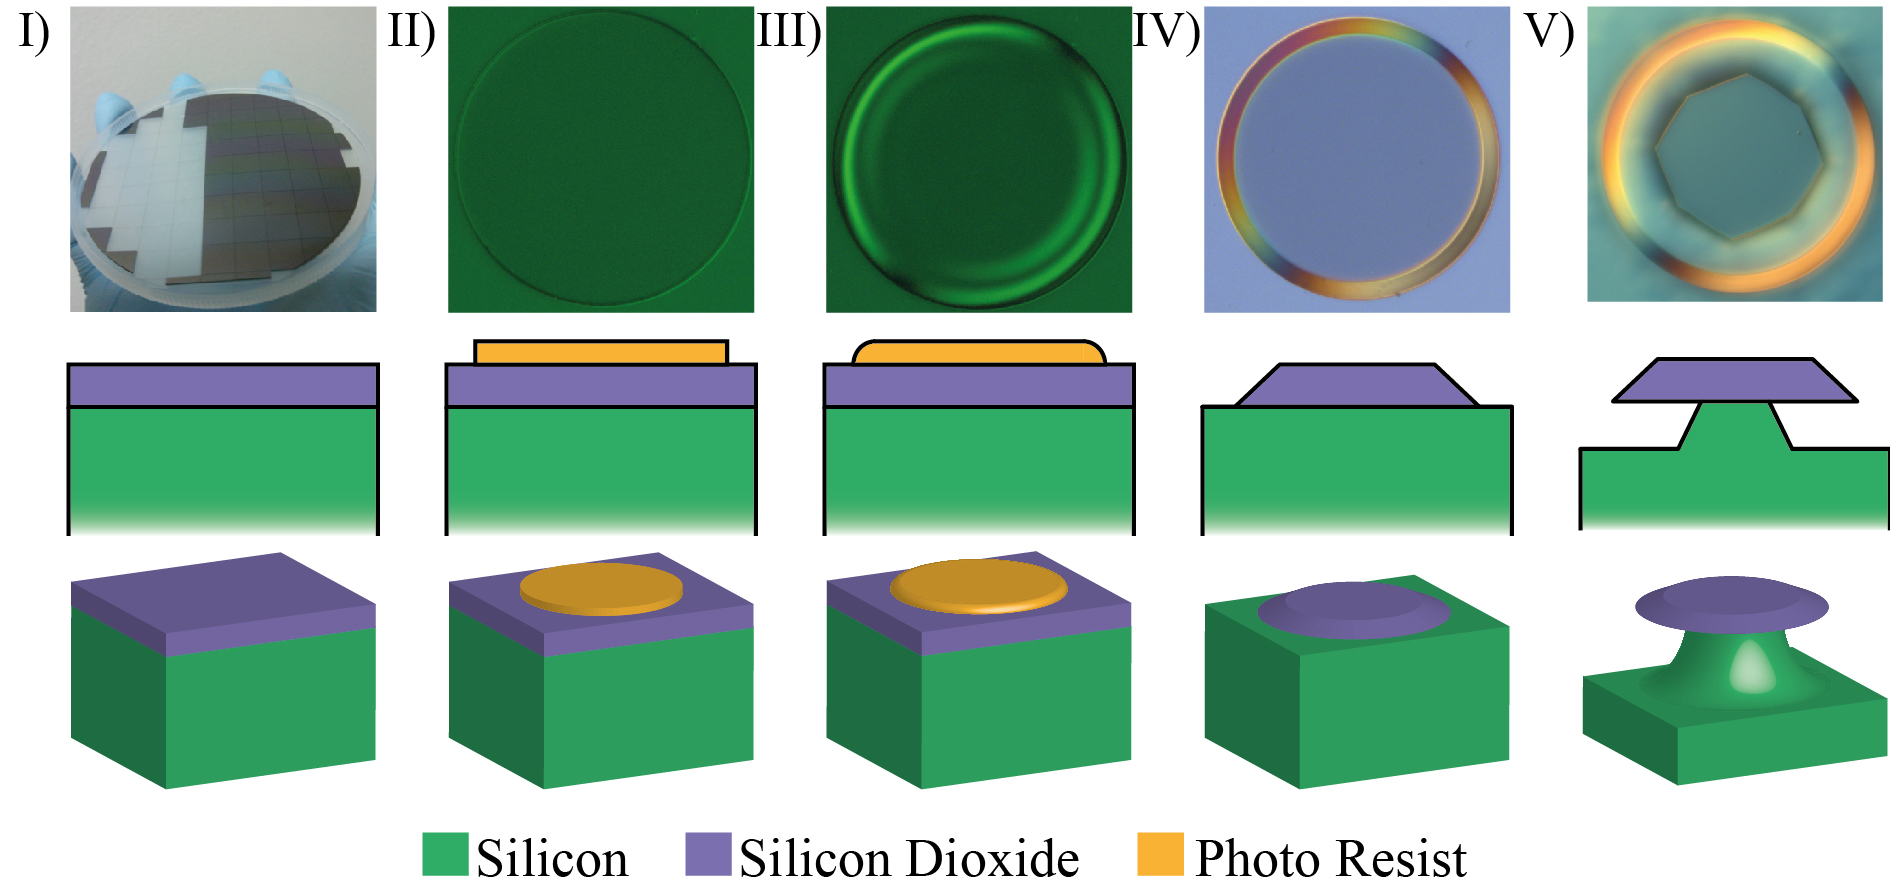
\includegraphics[width = 16cm]{figuras/Dissertation_fabrication_steps.jpg}
    \caption{\textbf{Steps of Fabrication:} The first row shows pictures taken in a optical microscopy. The second row shows a schematic draw of the layers. The last row show a perspective scheme.}
    \label{fig:fab_step}
\end{figure}

\section{Lithography}

In top-down microfabrication it is usually applied to transfer a pattern to a mask in order to protect the subtract during the etching process. 
\begin{figure}[!h]
    \centering
    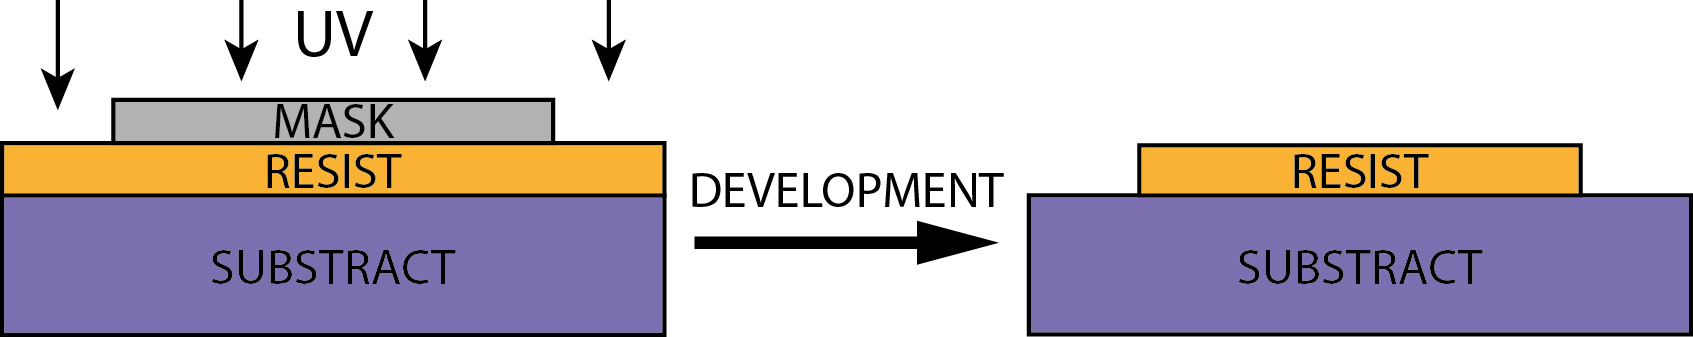
\includegraphics[width = 16cm]{figuras/Dissertation_litho.jpg}
    \caption{\textbf{Contact lithography}: A chrome mask is contacted with the resist and physically block the UV radiation, enabling to sensitize selectively and to transfer the mask pattern to the resist.}
    \label{fig:litho}
\end{figure}

Initially we deposit a photo sensitive resin, called resist. A chrome mask with the device pattern is used to cover-up the resist, then a UV light source is used to expose the uncovered resist, as schematically showed in Fig~\ref{fig:litho}. The UV light cause a chemical change in the resist that allows it to be removed using a specific solution, called developer. 

A crucial aspect in the lithography process is the adherence between the resist and the substrate. To fabricate this cavities we use a wet etching process, as we shall see below, which is very affected by the adherence. The Fig.~\ref{fig:adhrence_problem} 
shows the result of a etching with poor adherence, em some case the device totally vanish from the sample, and the process is not reproducible.
\begin{figure}[!hbt]
    \centering
    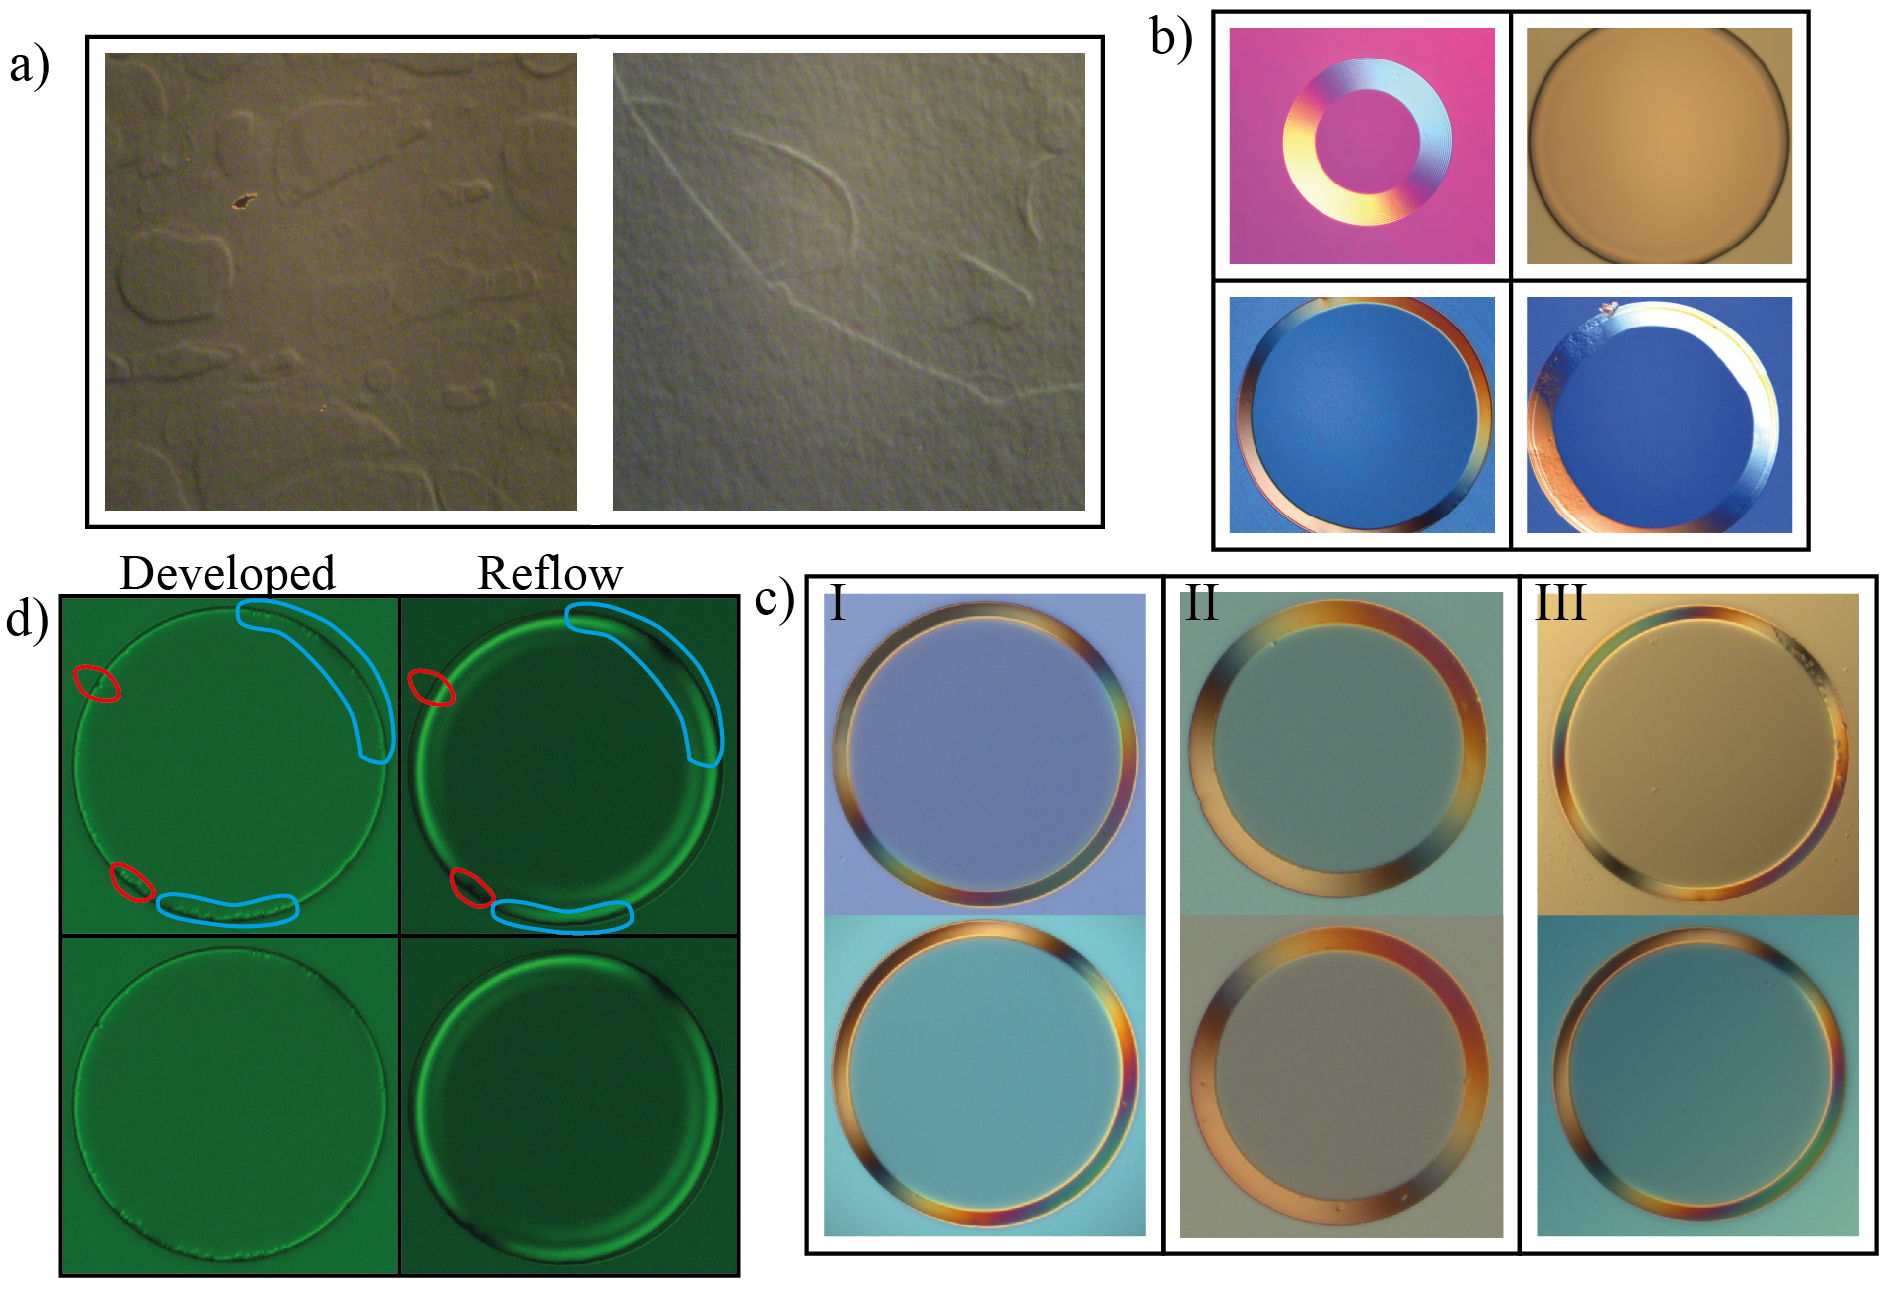
\includegraphics[width = 16cm]{figuras/Dissertation_etching_result.jpg}
    \caption{\textbf{a) Substrate Defect:} The irregularity in the surface of the substrate prevent a good adherence of the resist. \textbf{Comparison of Reproducibility: b)} Examples of different samples made with the same recipe using the commercial wafer; due to limitation on the optical microscopy, isn't possible to use a scale, however all images was made using the same magnification. \textbf{c)} Examples of different samples using the non-commercial wafer; each par of images was made using the same recipe, it shows that the result is consistent. \textbf{d) Reflow:}(top) Highlighted in blue defects suppressed by the reflow, in red defects that remains after the reflow. (bottom) Picture of the same cavity without the highlight to ease visualization.}
    \label{fig:adhrence_problem}
\end{figure}

In order to improve the adherence of the resist there are some cares that should be taken before the resist deposition. We have notice that the commercial wafer initially used as substrate present some irregularity in the surface, as show in Fig.~\subref{fig:adhrence_problem}{a}, this defects lead to a poor adherence and problems cited above. To solved it we used a non-commercial wafer grown by wet-oxidation. The reproducibility of the process presented a significant improvement, which can be seen in the comparation of the Fig.~\subref{fig:adhrence_problem}{b}. Besides that, a non aggressive organic cleaning is necessary to archive the good results presented.

The replication of the mask pattern in the resist after the development is highly accurate, which could be a problem since it will replicate the defects in the mask also, as can be easily spotted in Fig. A technique to attenuate this kind of defect is to heat the sample to the softening temperature of the resist, in this way the borders of the resist will reconstruct smoother~\needcit, this technique is called reflow. The result is shown in the Fig.~\subref{fig:adhrence_problem}{c}.

With a well deposited kinkiless resist we can etch the sample to fabricate the wedge disk cavities. 

\section{Etching}

In typical etching process, the resist act as a etch shield protecting the subtract from the etch. In this process, however, the resist orientate the etch direction by smoothly peel off during the etching. The Fig.~\ref{fig:wedeg_grow} illustrate how it occurs. Lets say, taking some linguistic liberty, that the interface between the solution and the silica act as a "etch source" of a spherical "etching wave". The "etch wavefront" appears under the resist, centered at the lower edge, when the etchant infiltrates between the resist, it peels off and a new "etch source" is created. A continuous adiabatic resist peeling leads to a straight wall with shallow wedge angle. %The result of a inhomogeneous resist peeling is showed in the Fig~\ref{fig:ethc_wrong}. 

\begin{figure}[!ht]
    \centering
    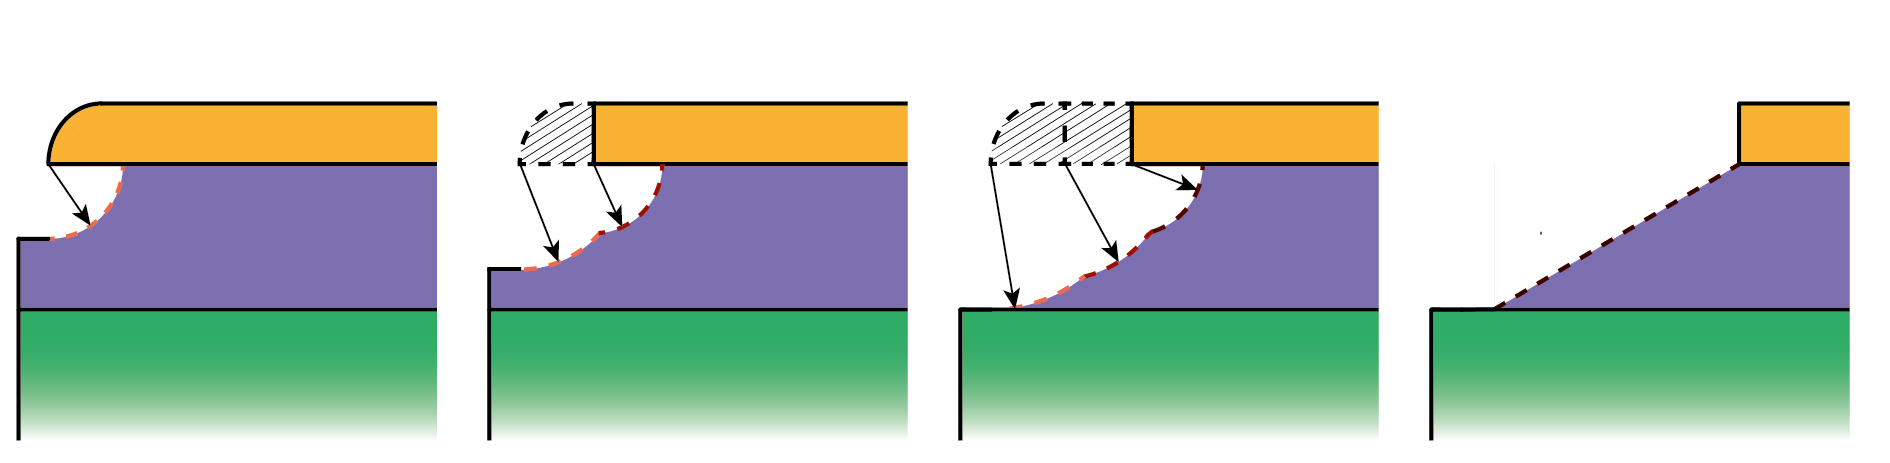
\includegraphics[width = 16cm]{figuras/Dissertation_etching.jpg}
    \caption{\textbf{Peeling Process Pictured:} The resist keep pilling off as long the sample is keeping in the etchant solution. A continuous process with small steps lead to a well defined wedge.}
    \label{fig:wedeg_grow}
\end{figure}

The reaction between the silica and the hydrofluoric acid occurs following the equation~\cite{Kang_2002} 
\cheeq{SiO2 + 4HF -> SiF4$_{(g)}$ + 2H2O}.
A buffered solution is used to maintain the solution concentration constant and decrease the etch rate, leading to a slower reaction which suppress the occurrence of abrupt defects contributing to a smooth surface, decreasing the scattering loss and enabling high Q cavities. However, a scanning electronic microscopy show unexpected defects in the cavities surface, as shows Fig.\subref{fig:ethc_wrong}{a}. This image was made using the initial commercial wafer, due to lack of time it wasn't possible to check if the new wafer solved this problem, thus, the origin of this problem is still unknown. 

Another common defect after the etching process is the rise of holes, especially in the wedge region. It is probable that the pressure between the mask and the resist in the contact lithography step creates microcracks that allow the etchant to infiltrate through the resist and etch the silica faster in this points, as pictured in Fig~\subref{fig:ethc_wrong}{b}, however a more detailed study would be necessary to prove this hypothesis. 

\begin{figure}[!ht]
    \centering
    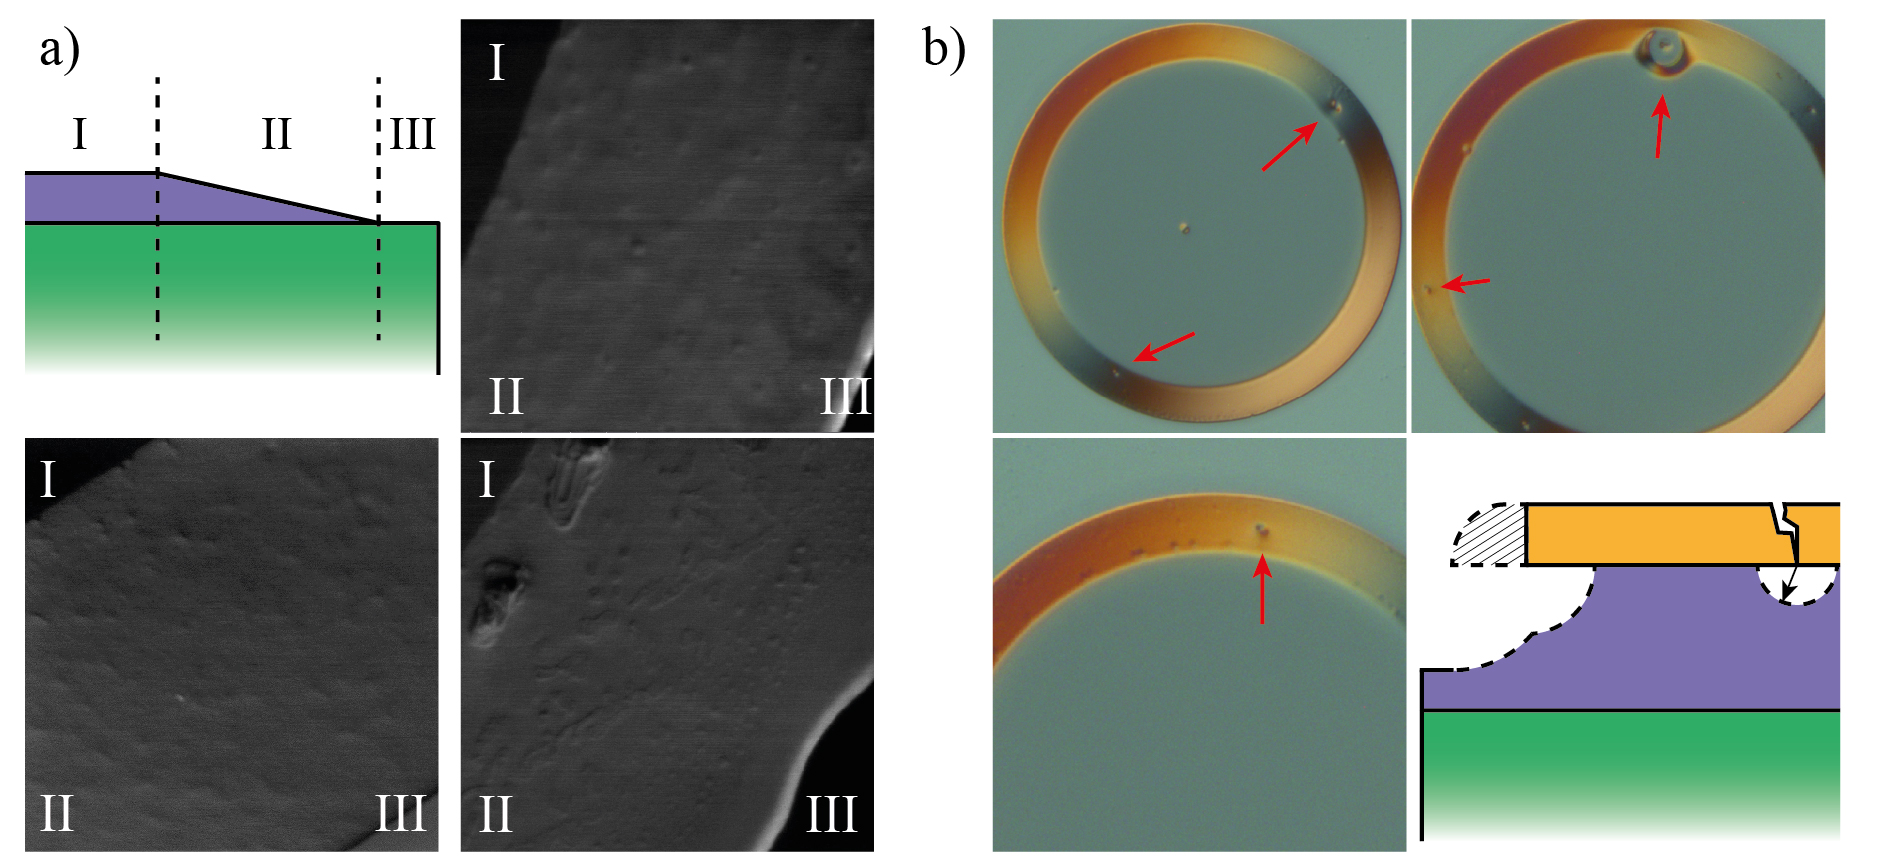
\includegraphics[width = 16cm]{figuras/Dissertation_etchin_def.jpg}
    \caption{\textbf{After Etching Defects:a)} Roughness at wedge surface. \textbf{b)} holes in the devices probable originated from micro cracks}
    \label{fig:ethc_wrong}
\end{figure}

The etching step build up the device, however they are fully in touch with the silicon layer. To improve the index contrast and enable the mode to be confined, we must release the cavity from the substrate, which is made by etching the silicon.

\section{Release}

The release procedure usually is made using a isotropic etch, otherwise the device would act as a mask. However, due to the crystalline characteristic of the silicon it is possible to apply a anisotropic etch, since the preferential direction is the atomic plan that goes under the device, leading to polygonal pedestal as can be seen in Fig~\subref{fig:release}{a}I and II.

The wet etch of the silicon occurs at presence of hydroxide that react with the silicon according with the reaction
\cheeq{Si + 2OH- + 2H2O -> Si (OH4)- + H2$_{(g)}$}
which is preferentially occurs at the (111) plane direction~\cite{Glembocki_1985}, enabling the releasing of the devices. For that we have test the etch using potassium hydroxide (KOH) and tetramethylammonium hydroxide (TMAH).

The compound \ce{Si(OH)4}, named orthosilicic acid, is aqueous and can also be obtained by the reaction\cite{madou2002fundamentals} 
\cheeq{SiO2 + 2H2O <=> Si(OH)4}
which mean that the etching of the silicon can also affect the silicon oxide device. In order to increase the selectivity of the process we have to adjust the concentration and temperature parameters of the solution~\needcit 

\begin{figure}[!b]
    \centering
    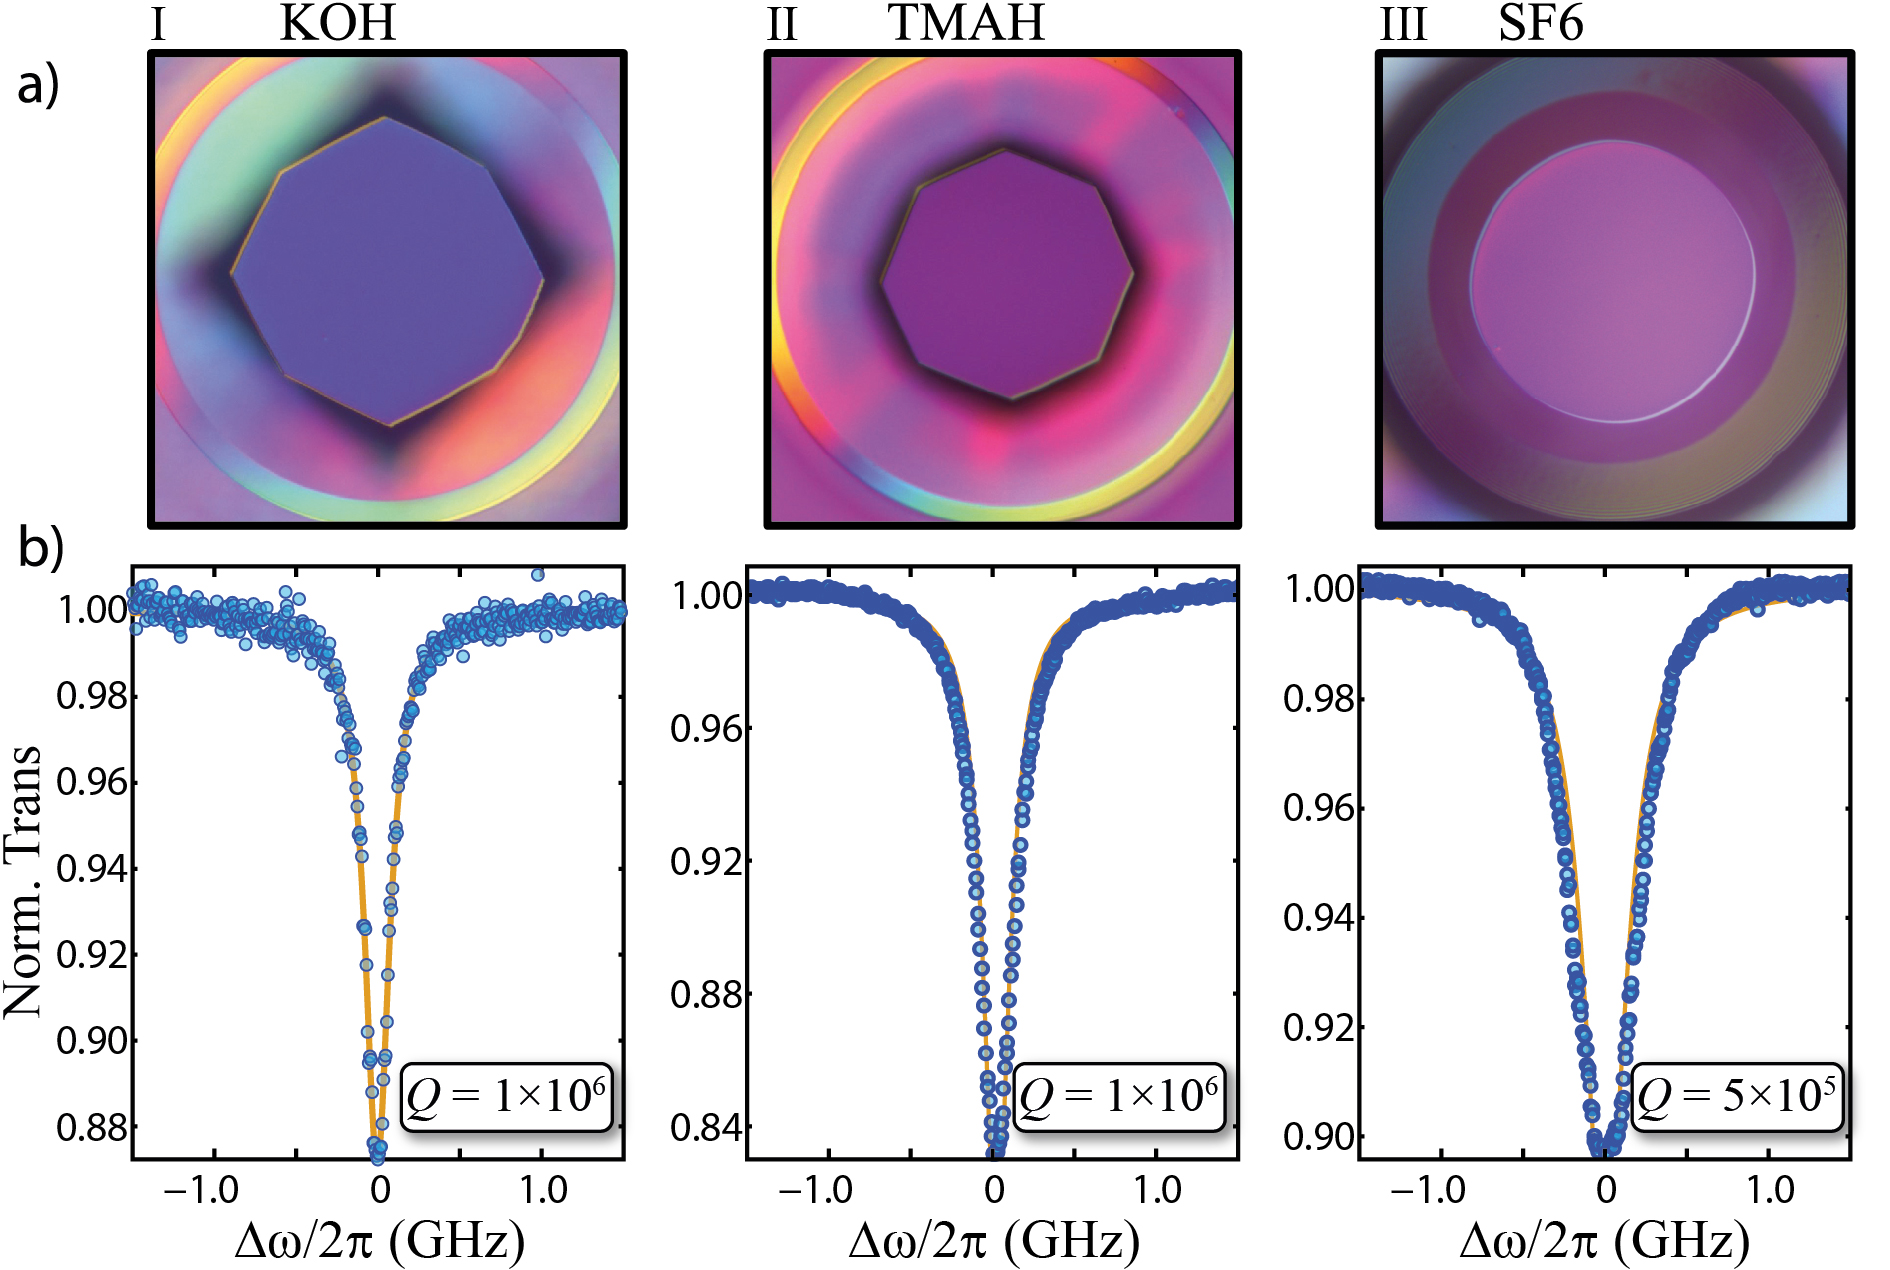
\includegraphics[width = 16cm]{figuras/Dissertation_release.jpg}
    \caption{\textbf{Release Process Comparation:a)} The initial difference between the anisotropic, KOH and THMA, and the isotropic release lies in the pedestal shape, that can introduce stress in the device surface, hence, introduce losses. \textbf{b)} To analyse the effect of the release in the losses, it was measured the maximum Q factor reached, the result don't show a considerable variation.}
    \label{fig:release}
\end{figure}
The polygonal shape of the pedestal could be introducing mechanical stress in the interface between the silica and the silicon, with would lead to a increase in the losses. In order to test this hypotheses a isotropic release process was test. The cavities was released by dry etch, using \ce{SF6}/\ce{O2} plasma~\cite{Eisele_1981}, leading to a pedestal as show in Fig~\subref{fig:release}{a}III. In the etch process we have, basically, two reaction occurring
\begin{subequations}
    \begin{alignat}{2}
        &\ce{Si + 4F& & -> SiF4}\label{etc:si}\\
        &\ce{SiO2 + 4F& & -> SiF4 + O2}\label{etc:sio}.
    \end{alignat}
\end{subequations}
However, the reaction probability to the reaction~\ref{etc:sio} is much lower than that of the reaction~\ref{etc:si}~\cite{Knizikevicius_2009}. The rigth set of parameters can lead to a high selective etching~\cite{Frederico_2003}. 
%https://www.sciencedirect.com/science/article/pii/S0921510797002171
 
The motivation for try different etching process is to determine what one causes less impact in the devices, once, was showed, all of then also etch silicon oxide. The result of each one is presented in the Fig. 

The parameter used to classify the cavities was the max reached Q factor. None of the process presented a high improvement. The Fig~\subref{fig:release}{b} brings the transmission for the mode with maximum Q factor. However, this test was done before we discovery the defects in the commercial wafer, in such way that the Q factor could already by limited early in the process. Due to practicality and reproducibility, we choose to do the release using TMAH.   
 
\section{Conclusion}

We found the main source of defects in or process, it was the defective commercial wafer, unfortunately it was found in a late stage of the project and it wasn't possible to revisited the other steeps to improve the fabrication results. 

It was possible to elaborate a fully reproducible recipe to fabricate wedge micro cavities in silicon dioxide at in-house facilities. We identified the key point of each step leading to a list of problems that need to be solved;
\begin{itemize}
    \item Lithography
    \begin{itemize}
        \item[$\ast$] Defects in the chrome mask is replicated in the resist, is required to fabricate a mask with least defect as possible. 
        \item[$\ast$] The pressure necessary to contact photolythography possible create micro cracks that allow the resist to infiltrate between the resist, damaging the device.
    \end{itemize}
 
    \item Etching
    \begin{itemize}    
        \item[$\ast$] The result after the etching must be checked using SEM.
    \end{itemize}
    
    \item Release
    \begin{itemize}
        \item[$\ast$] The comparation between release techniques should be redone.
    \end{itemize}
\end{itemize}

Follow this list may determine the way to improve our fabrication process till the state of art~\needcit. 





\chapter{Couple Mode Theory}
\label{chap:couple_mode}
%Descrição dos modos a1 e a3 considerando a perturbação de terceira ordem no autovalor. No final da sessão vou ter descrito a teoria do mapa de eficiência. Aqui uso como gancho a necessidade de saber os valores de $\kappa_e$ e $\kappa_i$ do visível e o valor de $J_3$ como motivação para todo o resto.  

The cavities we fabricate are designed to presents multiples optical modes. In this Chapter we shall study how the nonlinearity of the material affect this modes. Initially a infrared mode are excited using a external source, the third harmonic of the source act as a new source with the triple of the frequency in the neighborhood of a visible mode, leading to a couple behavior of this modes, this coupling can be described using the rate equation  

\section{Couple Rate Equation}
%
%From now on we are interested in optical mode with specific feature. Let's assume a mode with frequency $\omega_1$ at infrared, we want to know how it couple with a visible mode of frequency $\omega_3 = 3\times\omega_1+\delta$. 
%
%\begin{subequations}
%    \begin{alignat}{2}
%        \dot{a}_1 &= -\left(i\Delta_1 + i\omega_1 A_1|a_1|^2 + i\omega_1 A_{13}|a_3|^2 + \frac{\kappa_1}{2}\right)a_1 + \sqrt{\kappa^{(e)}_1}S_{in},\\
%        \dot{a}_3 &= -\left(i\Delta_3 + i\omega_3 A_3|a_3|^2+ i\omega_3 A_{31}|a_1|^2 + \frac{\kappa_3}{2}\right)a_3.
%    \end{alignat}
%\end{subequations}

The Eq~\ref{eq:rate_equation_bistable} give us the behavior of a single mode. For problems with low nonlinearity, when is possible to neglect terms of order $\left(\chi^{(n)}\right)^2$ and highers, the effect of the nonlinearity can be found using perturbation theory. 
\begin{equation}
    \frac{\delta\omega_\alpha}{\omega_\alpha} = \frac{1}{2}\frac{\bra{\vec{E}_\alpha}\delta\epsilon\ket{\vec{E}}}{\braket{\vec{E}_\alpha|\vec{E}_\alpha}} = \frac{1}{2}\frac{\int\vec{E}^*_\alpha\delta\vec{P}d^3\vec{r}}{\int \epsilon|\vec{E}_\alpha|^2d^3\vec{r}}
    \label{eq:perp_theory}
\end{equation}
Note that $\vec{E}_\alpha$ is the unperturbed electric field of the $\alpha$th mode, while $\vec{E}$ is the total electric field. 

For a generic problem $\delta\epsilon\ket{\vec{E}}=\ket{\delta\vec{P}}$ is the change in the polarization due to nonlinearity perturbation, as we are studding third order nonlinearity this perturbation can be write as $\delta\vec{P} = \epsilon\chi^{(3)}|\vec{E}|^2\vec{E}$. Our model assumes that there is only two different modes coupled, in such way that the total electric field is
\begin{equation}
    \vec{E} = \vec{E}_1+\vec{E}_3+c.c.
\end{equation}
From now on, the label $1$ refers to the model in the infrared and the label $3$ to the mode in the visible. 
The calculus of the Eq~\ref{eq:perp_theory} give rise to a total of sixty four terms for each one of the modes, however most of then are not of our interest. In order to filter this terms we will write the electric field with a explicit dependency of time $\vec{E}_\alpha(\vec{r},t) = a_\alpha(t) \vec{e}_\alpha(\vec{r})$. Considering the approximation of slowly variation, the amplitude $a_\alpha(t)$ can be considered as a harmonic function with frequency $\omega_\alpha$. Applying this trick, some terms of the Eq~\ref{eq:perp_theory} can be considered out of frequency and be neglected. The full expression for the perturbation for each mode is

\begin{eqnarray}
\frac{\delta\omega_1}{\omega_1} &=& -\frac{1}{8}\left[|a_1|^2\frac{\int\epsilon\chi^{(3)}
\Big(|\vec{e}_1\cdot\vec{e}_1|^2 + 2|\vec{e}_1\cdot\vec{e}_1^*|^2
\Big)d^3\vec{r}}
{\int \epsilon|\vec{e}_1|^2 d^3\vec{r}}\right. +\nonumber\\
&+&2|a_3|^2\frac{\int\epsilon\chi^{(3)}
\Big((\vec{e}_1\cdot\vec{e}_1^*)(\vec{e}_3\cdot\vec{e}_3^*)+|\vec{e}_1\cdot\vec{e}_3|^2+|\vec{e}_1\cdot\vec{e}^*_3|^2
\Big)d^3\vec{r}}
{\int \epsilon|\vec{e}_1|^2 d^3\vec{r}}+\nonumber\\
&+&\left.\frac{(a^*_1)^2a_3}{a_1}\frac{\int\epsilon\chi^{(3)}
\Big(3(\vec{e}^*_1\cdot\vec{e}_1^*)(\vec{e}^*_1\cdot\vec{e}_3)
\Big)d^3\vec{r}}
{\int \epsilon|\vec{e}_1|^2 d^3\vec{r}}\right]
\end{eqnarray}

\begin{eqnarray}
\frac{\delta\omega_3}{\omega_3} &=& -\frac{1}{8}\left[|a_3|^2\frac{\int\epsilon\chi^{(3)}
\Big(|\vec{e}_3\cdot\vec{e}_3|^2 + 2|\vec{e}_3\cdot\vec{e}_3^*|^2
\Big)d^3\vec{r}}
{\int \epsilon|\vec{e}_3|^2 d^3\vec{r}}\right. +\nonumber\\
&+&2|a_1|^2\frac{\int\epsilon\chi^{(3)}
\Big((\vec{e}_1\cdot\vec{e}_1^*)(\vec{e}_3\cdot\vec{e}_3^*)+|\vec{e}_1\cdot\vec{e}_3|^2+|\vec{e}_1\cdot\vec{e}^*_3|^2
\Big)d^3\vec{r}}
{\int \epsilon|\vec{e}_3|^2 d^3\vec{r}}+\nonumber\\
&+&\left.\frac{(a_1)^3}{a_3}\frac{\int\epsilon\chi^{(3)}
\Big(3(\vec{e}_1\cdot\vec{e}_1)(\vec{e}_1\cdot\vec{e}^*_3)
\Big)d^3\vec{r}}
{\int \epsilon|\vec{e}_3|^2 d^3\vec{r}}\right]
\end{eqnarray}

In order to normalize the amplitude in such way that $|a_\alpha(t)|^2$ is the energy stored in the $\alpha$th mode, we should normalize the electric field $\vec{e}_\alpha \rightarrow\vec{e}_\alpha/\int|\vec{e}_\alpha|^2 d^3\vec{r}$. Using this form, the perturbation can be linked with the rate equation making $\omega_\alpha \rightarrow \omega_\alpha + \delta\omega_\alpha$. We can factorize the expression based in the dependence of the amplitude. 

\begin{eqnarray}
\frac{\delta\omega_1}{\omega_1} &=& A_{11}|a_1|^2 + A_{13}|a_3|^2 + B_1\frac{(a^*_1)^2a_3}{a_1},\label{eq:ir_per}\\
\frac{\delta\omega_3}{\omega_3} &=& A_{33}|a_3|^2 + A_{31}|a_1|^2 + B_3\frac{(a_1)^3}{a_3}\label{eq:vis_per}.
\end{eqnarray}

%The rate equation for both modes are write as
Once identified all terms, we use the rotation frame approximation making $a_1 \rightarrow a_1e^{i\omega t}$ and $a_3 \rightarrow a_3e^{i3\omega t}$, with $\omega$ being the source frequency. Them we have 
\begin{subequations}
    \begin{alignat}{1}
        \dot{a}_1 &= -\left(i\Delta_1 + \omega_1i(A_{11} |a_1|^2 + A_{13} |a_3|^2) + \kappa_{1}\right)a_1 - i\omega_1 B_1(a^*_1)^2a_3 
        +\sqrt{2 \kappa^{(e)}_1}S_{in}
        \label{eq:taxa_ir_broad}\\
        \dot{a}_3 &= -\left(i\Delta_3 + \omega_3i(A_{31} |a_1|^2 + A_{33} |a_3|^2) + \kappa_{3}\right)a_3 - i\omega_3 B_3(a_1)^3.
        \label{eq:taxa_vis_broad}
    \end{alignat}
    \label{eq:rate_broad}
\end{subequations}
This move lead us to few new terms. Let's take a look to each one of them. First, we define $\Delta_1 = \omega_1 - \omega$ and $\Delta_3 = \omega_3 - 3\times\omega$. 

The terms $A_{\alpha\alpha}$ look like to the SPM term presented in Eq~\ref{eq:rate_equation_bistable}, in fact both are responsible for the same effect. 

The directly dependence of the refractive index with the intensity of the electric field is called the Optical Kerr effect. It is possible to show that due to third order nonlinearity, the refractive index can be write as~\needcit
\begin{equation}
    \text{n} = \text{n}_0 + 2\bar{\text{n}}_2|E|^2 
\end{equation}
If included in the wave equation, it lead to the same bistable behavior discussed before. The difference between Kerr bistability and thermotic bistability lies in the nature of both. The Kerr effect responds at a time scale faster than thermotic\needcit~ and have to due just with the material, meanwhile the thermotic bistability is a intrinsic behavior of the optical cavity and can be affect by both, material and geometry. However, at the specific experimental condition, we can not distinguish the individual contribution of each one in the transmission~\needcit, hence we consider just one SPM term that includes contributions of both, Kerr and thermotic. 

Futhermore, the Eqs~\ref{eq:rate_broad} present another similar term, with the form $A_{ij}|a_j|^2$. The effec of this term is exactly the one discussed before, but the bistability are generated due to the other optical mode, for both Kerr and thermotic~\needcit. This term are called Cross Phase Modulation (XPM). The expression for Kerr SPM and XPM can be take from the perturbation theory as 


\begin{subequations}
    \begin{alignat}{1}
        A_{ii} &= \frac{1}{8}\frac{\int\epsilon\chi^{(3)}
        \Big[|\vec{e}_i\cdot\vec{e}_i|^2 + 2|\vec{e}_i\cdot\vec{e}_i^*|^2
        \Big]d^3\vec{r}}{\Big[\int \epsilon|\vec{e}_i|^2 d^3\vec{r}\Big]^2},
        \\
        A_{ji} &= \frac{1}{4}\frac{\int\epsilon\chi^{(3)}
        \Big[|\vec{e}_i|^2|\vec{e}_j|^2 + |\vec{e}_i\cdot\vec{e}_j|^2+ |\vec{e}_i\cdot\vec{e}_j^*|^2
        \Big]d^3\vec{r}}{\Big[\int \epsilon|\vec{e}_i|^2 d^3\vec{r}\Big]\Big[\int \epsilon|\vec{e}_j|^2 d^3\vec{r}\Big]}.
    \end{alignat}
\end{subequations}

The other new terms are $B_1$ and $B_3$.% It is important to emphasize the fact that the amplitude $a_\omega$ is complex, so this term presents a real and a imaginary part, which act as a source term. 
We will call it the Coupling term, it is responsible for convert energy from one mode to the other. The expression for both, can be take from the perturbation theory as
\begin{subequations}
    \begin{alignat}{1}
        B_{1} &= \frac{3}{8}\frac{\int\epsilon\chi^{(3)}
        (\vec{e}_1^*\cdot\vec{e}_1^*)(\vec{e}_1^*\cdot\vec{e}_3)
        d^3\vec{r}}{\Big[\int \epsilon|\vec{e}_1|^2 d^3\vec{r}\Big]^{3/2}\Big[\int \epsilon|\vec{e}_3|^2 d^3\vec{r}\Big]^{1/2}},
        \label{eq:coupling_b1}
        \\
        B_{3} &= \frac{1}{8}\frac{\int\epsilon\chi^{(3)}
        (\vec{e}_1\cdot\vec{e}_1)(\vec{e}_1\cdot\vec{e}^*_3)
        d^3\vec{r}}{\Big[\int \epsilon|\vec{e}_1|^2 d^3\vec{r}\Big]^{3/2}\Big[\int \epsilon|\vec{e}_3|^2 d^3\vec{r}\Big]^{1/2}}.
        \label{eq:coupling_b3}
    \end{alignat}
    \label{eq:coupling}
\end{subequations}

%Using energy conservation $\frac{d}{dt}\left(|a_1|^2+|a_3|^2\right) = 0$ we can find that $\omega_1B_1 = \omega_3B^*_3$ 
In order to solve the Coupled Rate Equations Eq~\ref{eq:rate_broad} we will use a numerical method with the software Mathematica, the Appendix~\ref{app:numerical_met} treat about the method, now we are interested in the results. 

\section{Coupling Coefficient}

The first interesting result come from the coefficients $B_1$ and $B_3$, it told us how a infrared photon is scattered for the visible modes. The spatial dependence of the electric field is important as the coupling coefficient depends on the overlap integral between the modes defined as 
\begin{eqnarray}
J_3 = \frac{\int
        (\vec{e}_1\cdot\vec{e}_1)(\vec{e}_1\cdot\vec{e}^*_3)
        d^3\vec{r}}{\Big[\int \epsilon|\vec{e}_1|^2 d^3\vec{r}\Big]^{3/2}\Big[\int \epsilon|\vec{e}_3|^2 d^3\vec{r}\Big]^{1/2}}
\end{eqnarray}

Before to simulate the modes to calculate the overlap integral let's consider the symmetry of the problem. The WGM presents a harmonic dependence in the azimuthal coordinate, thus enable us to write the electric field as $\vec{e_\alpha}(\vec{r}) = \vec{e_\alpha}(r,z)e^{-im_\alpha\theta}+c.c.$ which lead to a overlap integral with the form
\begin{equation}
    J_3 = \frac{\iint
        (\vec{e}_1(r,z)\cdot\vec{e}_1(r,z))(\vec{e}_1(r,z)\cdot\vec{e}^*_3(r,z))
        drdz}{\Big[\int \epsilon|\vec{e}_1|^2 d^3\vec{r}\Big]^{3/2}\Big[\int \epsilon|\vec{e}_3|^2 d^3\vec{r}\Big]^{1/2}} \int_0^{2\pi} 2\pi \theta \sin\left(\Delta m \theta\right)   d\theta
    \label{eq:overlap_j3}
\end{equation}
We define $\Delta m = m_3 -3\times m_1$. 

The result of the integral at far right is a Sinc function of $2\pi\Delta m$. Due to the symmetry of our problem, the value of any $m_\alpha$ is a integer, thus $\Delta m$ is also a integer. The value of the Sinc function goes to zero for any integer $\Delta m$ different from zero, as show in Fig~\subref{fig:toy_model}{a}, therefore the coupling of two modes due third order nonlinearity occurs just if $m_3 = 3\times m_1$, hence $k_3 = 3 \times k_1$. This relation between the constant of propagation is one of the conditions necessary for phase matching, as saw in Chapter~\ref{chap:nonlin_pol}. In order to reach the phase matching we need to set the relation between the frequency of the modes, this is a important statement as we shall see next.  

\begin{figure}[t]
    \centering
    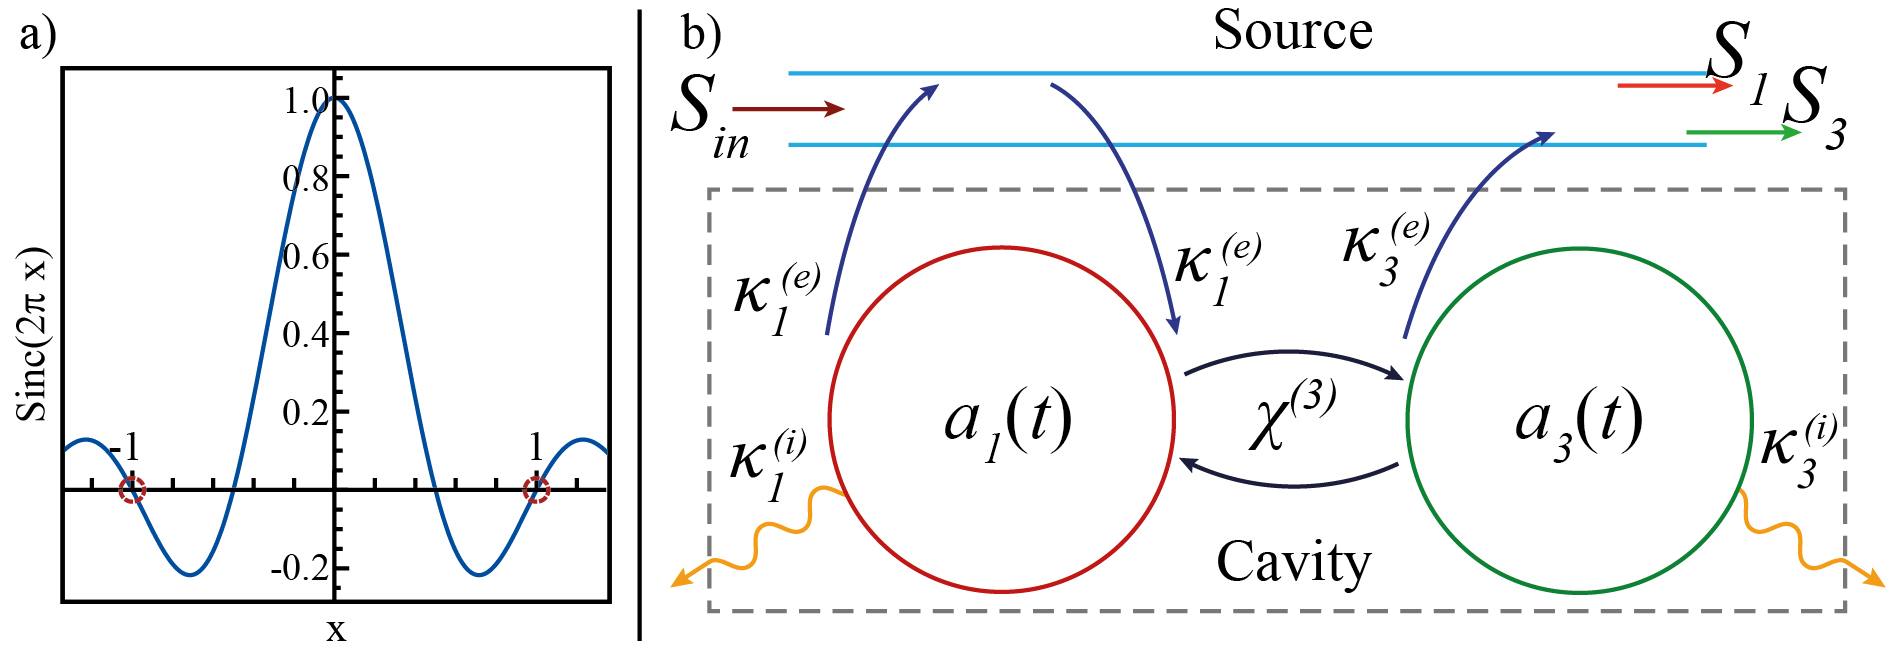
\includegraphics[width=16cm]{Dissertation_coupled_mode.jpg}
    \caption{\textbf{a) Sinc function:} The Sinc function of $2\pi x$ goes to zero for any integer $x$, but for $x=0$. \textbf{b) Lumped Model:} Our system are compound by a Cavity with two modes, both couple with bus waveguide that carry the input wave. The intrinsic loss and couple loss are different for each mode. The coupling between the modes occurs due to third order nonlinearity. }
    \label{fig:toy_model}
\end{figure}

\section{Numerical Results}

We will solve the Coupled Rate Equation using numerical methods. Our problem can be modeled as show in Fig~\subref{fig:toy_model}{b}. A system compound by a cavity with two modes, one in infrared ($a_1$) and one in visible ($a_3$), a input wave ($S_{in}$) with frequency near of the infrared mode. Both modes couple with the same bus waveguide that carries the input wave. The output waves are defined as 
\begin{subequations}
    \begin{align}
        S_1 &= S_{in} - \sqrt{\kappa^{(e)}_1}a_1\\
        S_3 &= \sqrt{\kappa^{(e)}_3}a_3
    \end{align}
\end{subequations}

Initially, lest solve the Eq~\ref{eq:rate_broad} assuming phase matching between the modes, that is, lets consider $\omega_3 = 3\times\omega_1$. The Fig~\subref{fig:temporal_solution}{a}
brings a well know bistable curve for the infrared mode (Red) while the Fig~\subref{fig:temporal_solution}{b} 
shows a slightly deformed lorentzian curve for the visible mode. This curve shape are true just if we assume that $\omega_3 = 3\times\omega_1$, which is not true due to the dispersion of the modes. A more general model assume that $\omega_3 = 3\times\omega_1 + \delta\omega$, in such case, the shape of the curve can be totally changed in function of the value of $\delta\omega$, we call this term frequency detuning. The Fig~\subref{fig:temporal_solution}{c}
shows some case. 

\begin{figure}[!h]
    \centering
    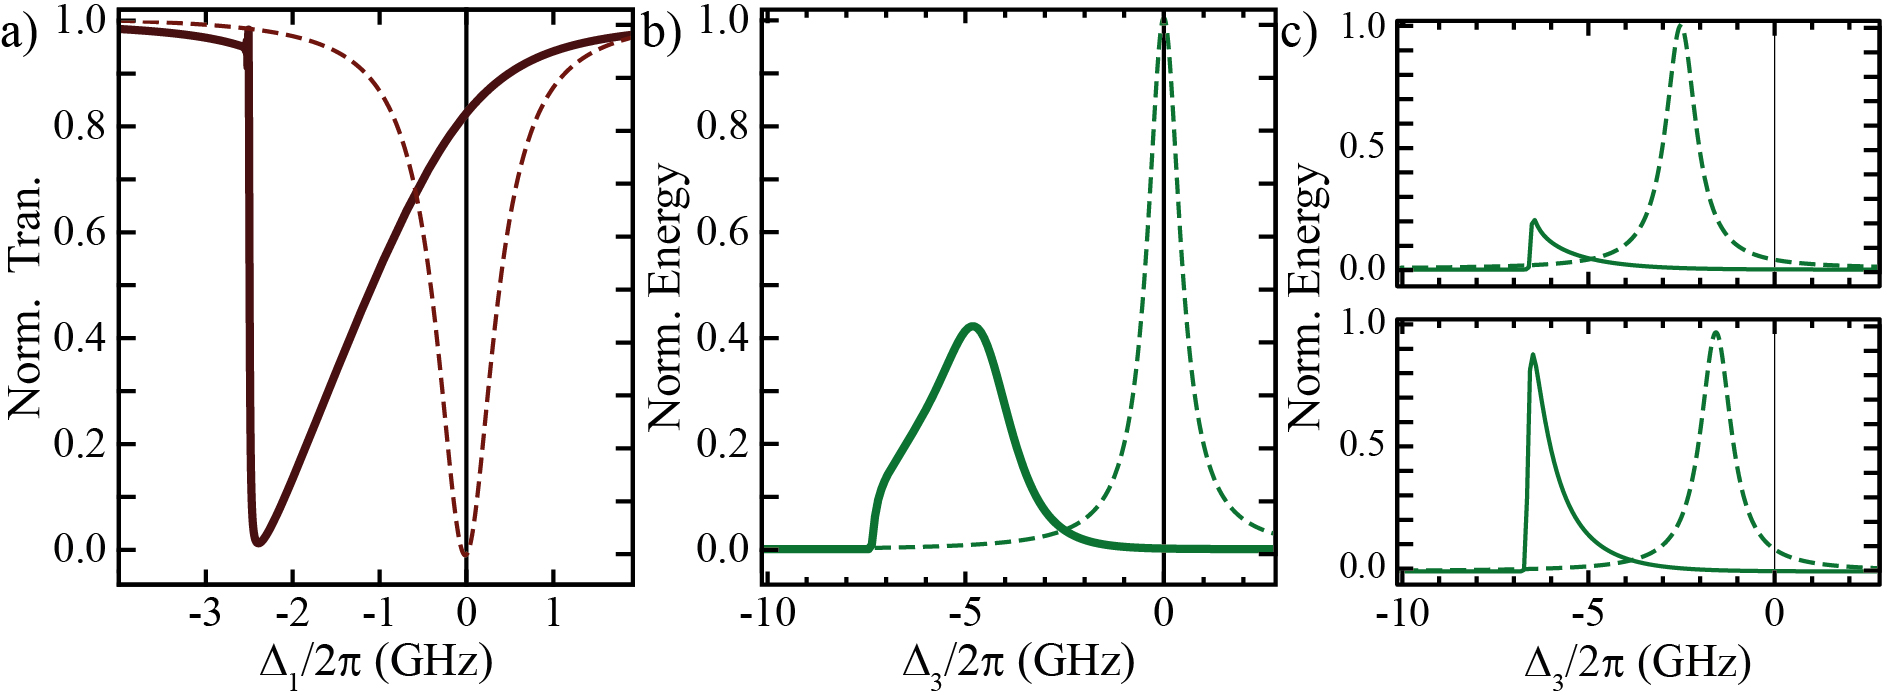
\includegraphics[width=16cm]{Dissertation_thg_solution.jpg}
    \caption{\textbf{Output in Function of the Detuning. a)} The solid line is the infrared transmission. The dashed line represents the initial state of the infrared mode. \textbf{b)} The solid line is the collected visible power (normalized by the optimal value). The dashed line represents the initial state of the visible mode. For this case, the frequency detuning is zero. \textbf{c)} Results for different frequency detuning. Upper $\delta\omega = 2\pi\times2.5$~GHz. Lower $\delta\omega = 2\pi\times1.5$~GHz, which is the close of the optimal case.}
    \label{fig:temporal_solution}
\end{figure}
This dynamics occurs due to the SPM and XPM terms. The displacement from the initial frequency are different for each mode which lead to different phase relation between the modes as long the source frequency is sweep. 

As we saw we Chapter~\ref{chap:optical_cavity} the displacement is direct related with the source power. A careful look to the solution for the Couple Rate Equation show that is always possible to find a situation, tuning both $\delta\omega$ and the power, that lead to a phase matching between the modes at the resonance. In this situation the conversion from the infrared to the visible are optimal. The frequency detuning can be set by changing the temperature of the cavity. 

The refractive index of the material is a different function of the temperature for which frequency~\needcit, thus changing the temperature of the hole cavity will lead to a different displacement for the frequency infrared than for the visible. 

Let's assume now that for any input power we are able to find a temperature that lead the phase matching to occurs at the resonance. This assumption is similar to assume that the SPM, XPM and frequency detuning are null in the Eq~\ref{eq:rate_broad}. The Fig~\subref{fig:power_solution}{a}
show the value of the ration between the collected visible power and the input power ($|S_3|^2/|S_{in}|$), which we define as Net Efficiency, in function of the input power. We are able to spot a critical power that lead to a maximum Third Harmonic Generation Net Efficiency. Moreover, this maximum is very stable in function of the power, the inset of Fig~\subref{fig:power_solution}{a} show that a variation of hundreds of Watts lead to a variation hundredth of the efficiency. For a specific scenario it is possible to reach a total conversion of photons from the infrared to the visible, the Fig~\subref{fig:power_solution}{b} shows the result considering this condition. 

\begin{figure}[h]
    \centering
    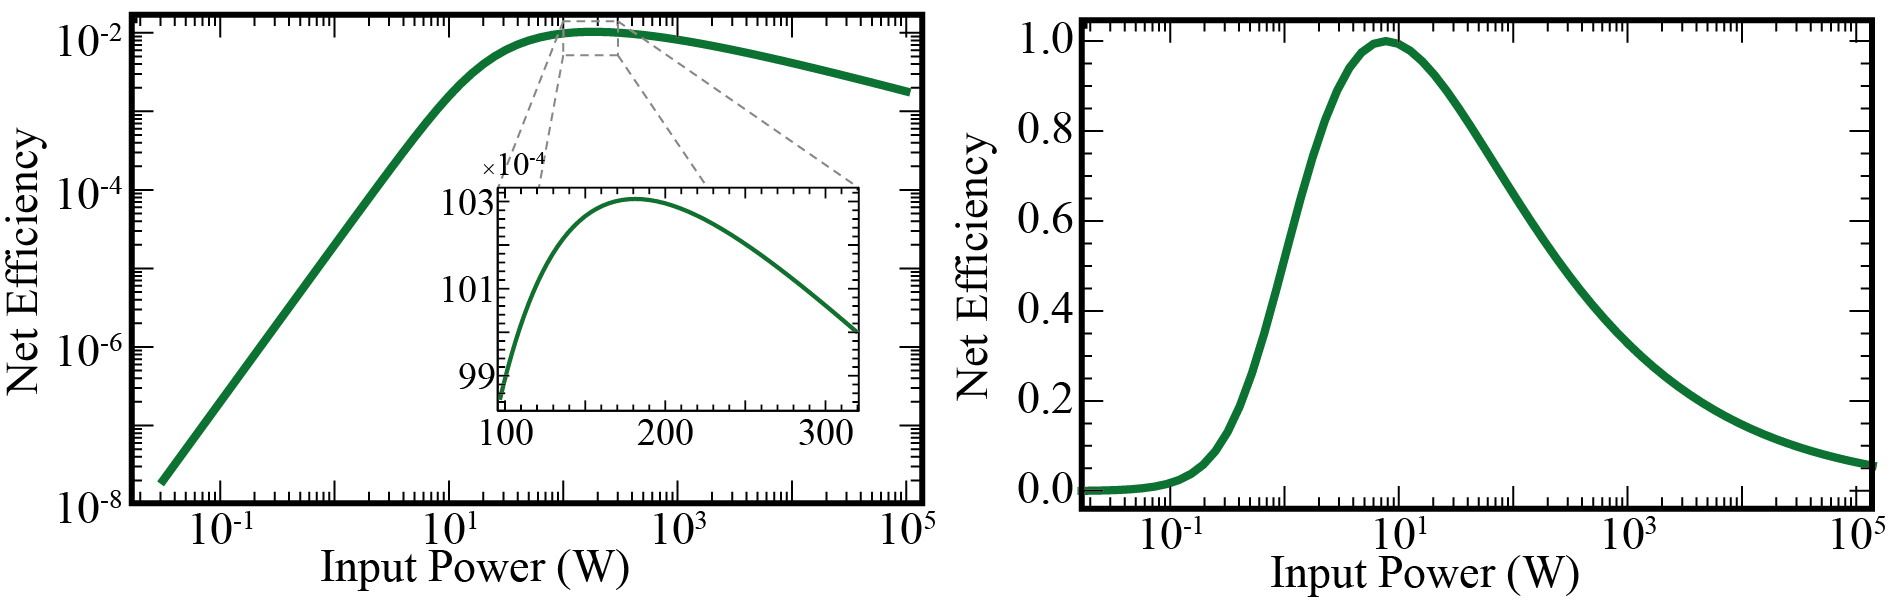
\includegraphics[width=16cm]{Dissertation_thg_eff.jpg}
    \caption{\textbf{Third Harmonic Generation Net Efficiency:} \textbf{a)} Numerical solution considering the values of the parameters close of the real system. \textbf{Inset:} Close look on the peak of efficiency. \textbf{b)} Numerical solution considering $\kappa^{(e)}/\kappa^{(i)} = 10^3$ for both, infrared and visible modes.}  
    \label{fig:power_solution}
\end{figure}

The most important assumption to reach a total conversion scenario is that the couple rate $\kappa^{(e)}$ must be much high than the loss rate $\kappa^{(i)}$ for both, infrared and visible, which lead to a engineer problem. Our coupling system, a tapered optical fiber, is optimized for the infrared mode, so the coupling with the visible mode is weak.

\section{Conclusion}

In this Chapter we have applied perturbation theory in order to develop a Rate Equation that couple two modes due to third order nonlinearity. This procedure lead us to few new terms, two phase modulation terms, self and cross (SPM and XPM), and the couple terms $B_1$ and $B_3$.

The overlap integral J3, Eq~\ref{eq:overlap_j3}, lead to the relation $m_3 = 3\times m_1$ for the coupled modes, which is necessary for phase matching. Meanwhile, the SPM and XPM displace differently each mode, leading to a frequency detuning of the modes. Nevertheless, as the displacement is a function of both, PM terms and the power, is possible to set specific values of power and initially detuning that lead to a perfect phase matching in the resonance frequency. 

If we consider a situation where the system is always in phase matching, the solution of the Coupled Rate Equation show a critical power wheres the efficiency of Third Harmonic Generation is maximized. This maximum occurs in a large band of power.

In order to verify the validation of this theoretical results, we proposed some set of experiments. The following Chapter shall treat this subject.  
\chapter{Experimental Methods}
%Os experimentos são descritos aqui. 
In order to compare experimental results with the theoretical prevision we must measured two parameters in the Eq.\ref{eq:taxa_ir_broad} and \ref{eq:taxa_vis_broad}. First we need to characterize the visible mode by measure the losses $\kappa^(i)_3$ and $\kappa^(e)_3$; we have apply two different complementary techniques for that. The second important parameter is the Coupling terms $B_1$ and $B_3$; the challenge lays in the calculation of the overlap integral, as defined in Eq~\ref{eq:overlap_j3}, since it is necessary to identify the optical modes related in the THG. With this values in hand, we must be able to compare the theoretical and experimental results. 

However, first of all, the main experiment in this dissertation is the generation of third harmonic in optical microcavities. Lets star by there. This Chapter present a scientific description of the experiments, meanwhile a technical overview is presented in the Appendix~\ref{app:experiment}

\section{Third Harmonic Generation in Optical Microcavities}

The experiment is done with a setup quite similar to the one used in the optical characterization of infrared modes, show in Fig~\subref{fig:exp_mode_charac}{a}, with the inclusion of a wave modulator, a Erbium Doped Fiber Amplifier and a free space setup in the output to split the infrared (which was high powered) from the third harmonic.
\begin{figure}[h!]
    \centering
    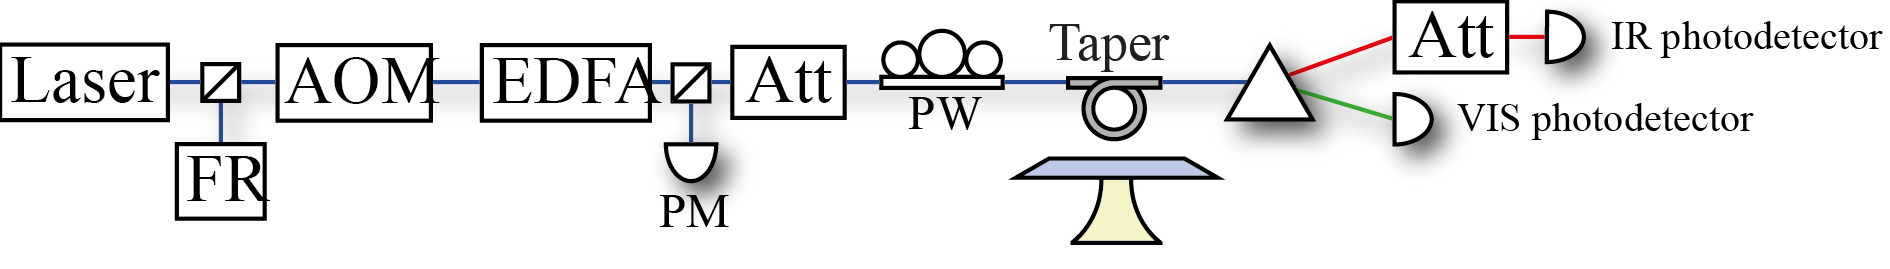
\includegraphics[width = 16 cm]{figuras/Dissertation_thg_setup.jpg}
    \caption{Experimental Setup: A infrared tunable Laser is modulated by a Acousto-optic Modulator (AOM) and amplified by a Erbium Doped Fiber Amplifier (EDFA) up to tens of watts. A Frequency Reference (FR) is used to precisely determine the frequency of the source, attenuator (att.) and paddle wheels are used to control the input power and polarization. The infrared part is splitted from the visible by a prism.}
    \label{fig:thg_setup}
\end{figure}

%in this paragraph I will talk about how to amplify the optical power
As seen in Chapter~\ref{chap:nonlin_pol}, to observe third order effects it is needed a power higher than the used in transmission experiment. To reach power high enough to the experiment a Erbium Doped Fiber Amplifier is applied, which amplifies the optical power to around $40$ dBm, to reach even higher power, the input wave is modulated in pulses with width of $400$~ns and duty cycle of $40$~$\mu$s using a Acousto-optic Modulator. 

The amplified power is monitored using a beam splitter. A fentosecond detector able to solve the pulse format enables to measured the power in function of time with the aid of a oscilloscope. The input power is controlled using a Attenuator, to keep the power measured by the IR photodetector at constant range another Attenuator is add to the circuit, the sum of the attenuation in both is keep constant.  

The experiment is done by sweep the frequency of the source and monitoring the power at the VIS photodetector. The result of the experiment is the power in visible band in function of the frequency of the source, as show in Fig.~\ref{fig:thg_broad_map}, each peak corresponds to a scenario wheres the condition to third harmonic generations, as sens in Chapter~\ref{chap:couple_mode}; this result was obtained as a preliminary result with the initial defective wafer. 
\begin{figure}[h]
    \centering
    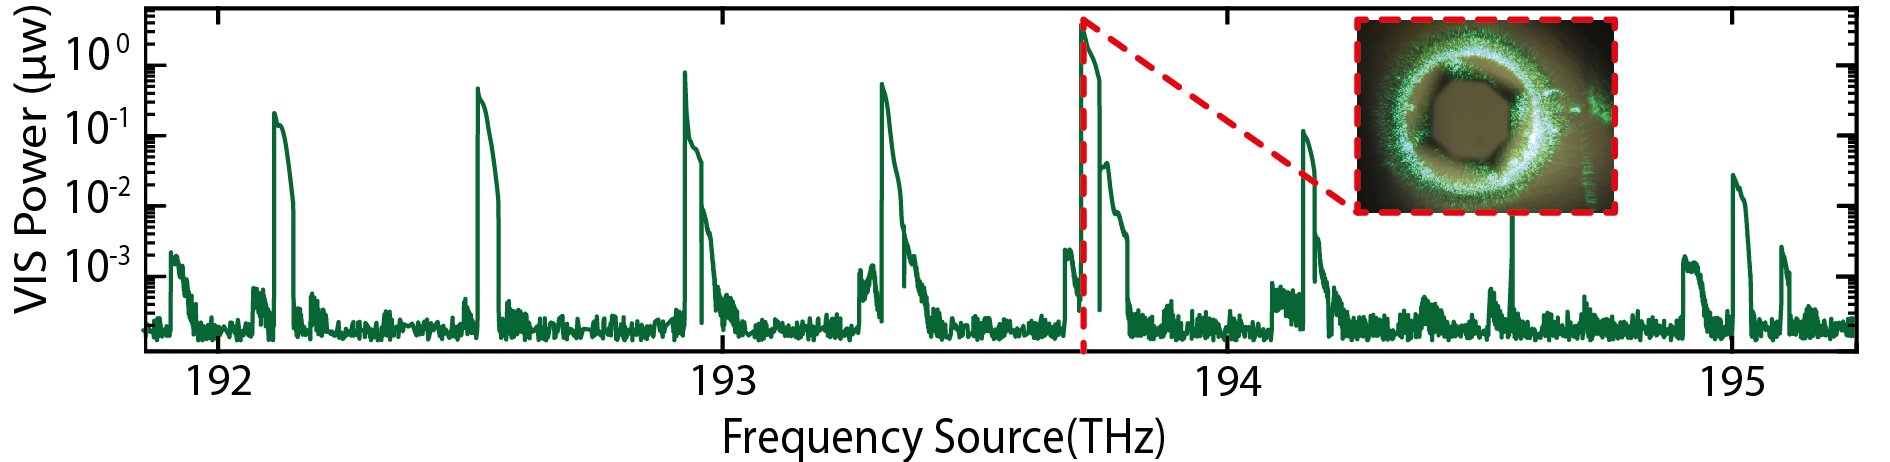
\includegraphics[width = 16cm]{figuras/Dissertation_thg_broad.jpg}
    \caption{Caption}
    \label{fig:thg_broad_map}
\end{figure}

The shape of the THG curves is significantly different of those predicted in the Fig.~\ref{fig:temporal_solution}, this is due to the interference between neighboring infrared modes. As the coupling between the cavity and the source must be high in in order to collect more TH, the amount of excited IR modes id high enough to produce a dirty transmission spectrum. 

Now we are interested in control the phase matching condition between the modes by change the phase detuning $\delta_\omega$. To change the phase detuning we shall vary the sample temperature and due to a dynamics similar to the presented in the Eq~\ref{eq:termooptc_change}; however, with a external heat source instead of internal one; therefore the Eq~\ref{eq:pertubation_bistaliti_cavity} can by write as 
\begin{equation}
    \frac{\Delta\omega_\alpha}{\omega_\alpha} = \frac{d\text{n}_\alpha}{dt}\Delta T \rightarrow \Delta\delta_\omega = \left(\omega_3\frac{d\text{n}_3}{dt} - 3\omega_1\frac{d\text{n}_1}{dt}\right)\Delta T
    \label{eq:temperature_mode_variation}
\end{equation}
the frequency displacement due to the sample temperature is different for each band, leading to a variation in the initial phase detuning, even don't knowing the initial phase detuning $\delta_0$ it is possible to calculate the variation in the phase detuning in function of the temperature and compare the effect over the third harmonic generation. 

The experimental result can be quantitatively compared with the numerical solution of the Eq~\ref{eq:taxa_ir_broad} and Eq~\ref{eq:taxa_vis_broad} for different values of $\delta_\omega$. The result is presented in Fig.~\ref{fig:thg_control_phase_det}. This measurement was made using the piezo frequency control of the laser, preventing the infrared mode to interfere with the neighbors, another technique was to slight increase the diameter of the tapered fiber, in relation with the Fig.~\ref{fig:thg_broad_map}, leading to a decrease in the amount of visible power collected. Another important difference is the use of samples fabricated with lab grown wafer.
\begin{figure}[!h]
    \centering
    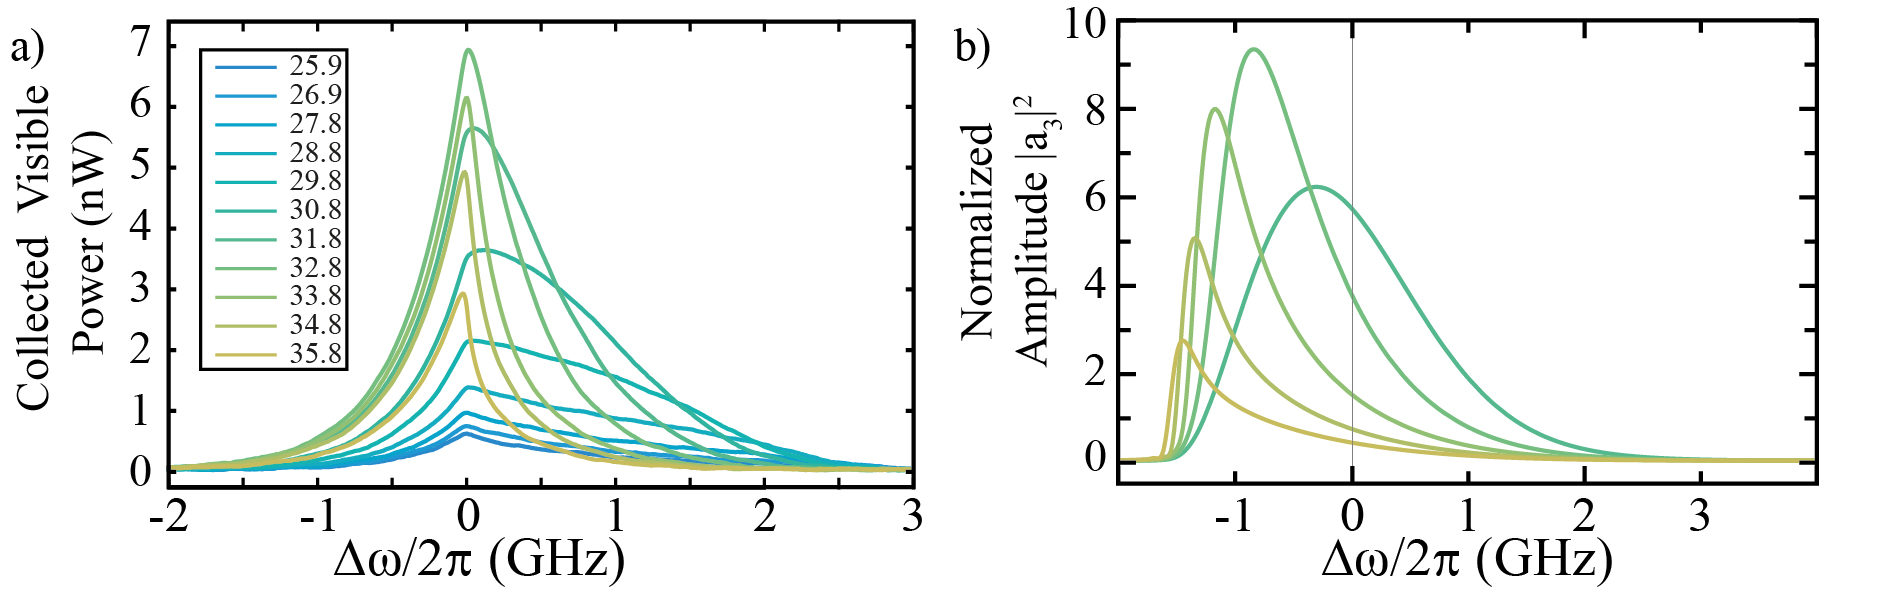
\includegraphics[width = 16cm]{Dissertation_phase_detuning_comp.jpg}
    \caption{Caption}
    \label{fig:thg_control_phase_det}
\end{figure}

In order to produce a quantitative comparation we need to measured the parameters cited above.  

\section{Optical Characterization at Visible Band}

The main challenge in characterize the cavity in the visible band is the lack of a tunable visible laser, which could be used as described in the Sections~\ref{sec:optical_char}. As we do not have access to a visible tunable laser, we need to apply a different techniques, two to be precise. One technique use the transmitted light from a external source, slightly similar from the infrared characterization, the other one use the third harmonic internally generated. 

\subsection{Transmission Characterization}

This experiment is based on the Eq~\ref{eq:single_mode_transmission}, wheres the Detuning $\Delta_3$ (do not mistake with the phase detuning $\delta_\omega$) was defined $\Delta_3 = \omega_3 - \omega$. The source used was a visible green laser ($532$~nm) with fixed frequency; therefore, in order to compute the transmission spectrum we vary the resonance frequency $\omega_3$ by change the sample temperature, according with the Eq.~\ref{eq:temperature_mode_variation} we can write 
\begin{equation}
    \Delta_3 = \omega_3\frac{d\text{n}_3}{dT}\Delta T.
\end{equation}
To determine the $\Delta T$ an infrared mode was used as probe, the details of the procedure can be find in the Appendix~\ref{app:experiment}.

The Fig.~\ref{fig:mode_char_trans} shows the result of the experiment. An infrared mode was characterize using the same procedure, as shown in Fig~a, where we can calculate the losses, $\kappa_1^{(i)} = 940\pm 50$~MHz and $\kappa_1^{(e)} = 180 \pm 6$~MHz, them we compare with the typical characterization (as described in Chapter~\ref{chap:optical_cavity}), show in Fig.~, we have measured $\kappa_1^{(i)} = 910\pm 20$~MHz and $\kappa_1^{(e)} = 173 \pm 2$~MHz, which showed a good agreement between the methods.
\begin{figure}[!h]
    \centering
    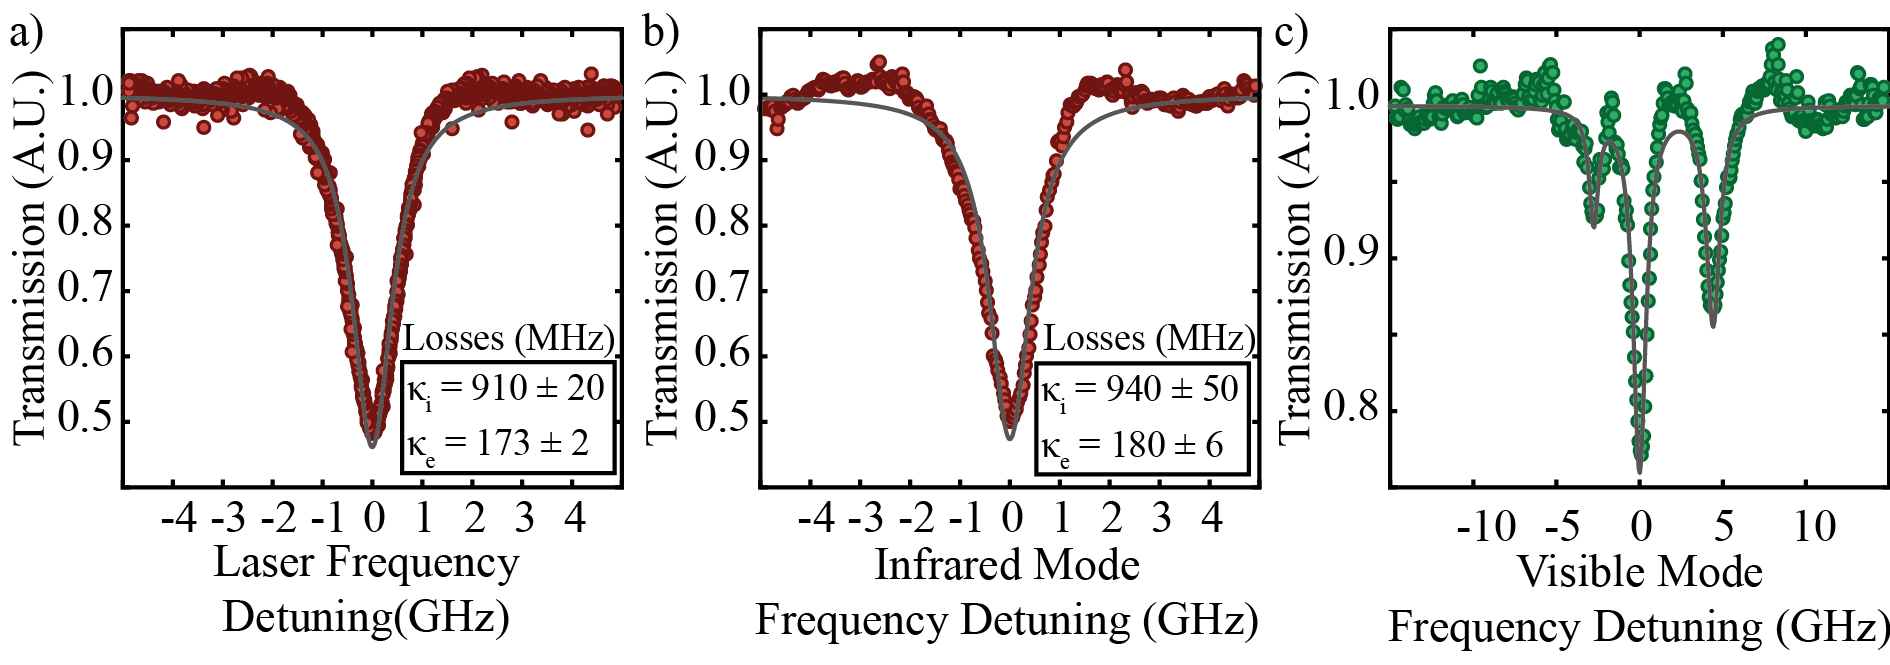
\includegraphics[width = 16cm]{Dissertation_char_vis_trans.jpg}
    \caption{Caption}
    \label{fig:mode_char_trans}
\end{figure}

The results for the visible mode is shown in the Fig~. It was possible to identify three different modes which was fitted with a variation of the Eq~\ref{eq:single_mode_transmission} to include the neighbors~\needcit. We have found the values
\begin{table}[h]
\centering
\begin{tabularx}{8cm}{c|c|c|c}
Modo & $\kappa_i$ (MHz) & $\kappa_e$ (MHz) & $Q_i$ ($10^5$) \\ 
\hline                               
1 &$700\pm200$&$12\pm2$&$9.0\pm2.0$\\
2 &$870\pm60$&$59\pm3$&$6.6\pm0.4$\\
3 &$950\pm90$&$37\pm2$&$6.1\pm0.5$
\end{tabularx}
\caption{1}
\end{table}

It is important to notice that the measured modes are out of band where we have measured third harmonic as the fundamental mode for this visible modes lies around the $1596$~nm, out of the EDFA band; however, this result bring us a strong feeling about the coupling rate between the visible modes and the source. The bus waveguide was designed for coupling infrared modes, which lead to a poor coupling for visible mode, as demonstrated in the numerical solution, Appendix~\ref{app:numerical_met}, the amount of visible light collected is strong dependent on the coupling, this result explain the low collected power presented in the Fig..

This technique characterize both $\kappa_3^{(i)}$ and $\kappa_3^{(e)}$, although it do not characterize a mode that we can measure third harmonic. The next technique use the generation of third harmonic to measures the losses, so, we necessary will be looking for a mode the interest band, in exchange, it will only be possible to measure the total loss. 

\subsection{Third Harmonic Generation Characterization}

Lets introduce a set of assumptions in order to rewrite the Eq~\ref{eq:taxa_ir_broad} and \ref{eq:taxa_vis_broad}. First, consider the steady state, $\dot{a}_\alpha = 0$, also lets consider that the system is in the resonance of the infrared, $\Delta_1 = \omega_1(A_{11}|a_1|^2+A_{13}|a_3|^2)$ for last we assume that the $a_3$ amplitude is much smaller than $a_1$, then we can write the energy in the visible mode as
\begin{equation}
    |a_3|^2 = \frac{|\omega_3 B_3 (a_1)^3|^2}{\left(\kappa_3\right)^2 + \left(\delta_0 - 3(A_{31}-A_{11})|a_1|^2\right)^2}
    \label{eq:thg_phase_mismatch}
\end{equation}

The assumption of resonance with the infrared is important to consider all parameters independents of the phase detuning, which lead to a Lorentzian function for the energy stored in the visible mode with the phase detuning as variable. Using the same procedure as before to vary the phase detuning and measuring the third harmonic power generated in the resonance of infrared is possible to determine the total loss $\kappa_3$. The result is shown in the Fig.~\ref{fig:mode_char_thg}.
\begin{figure}[!h]
    \centering
    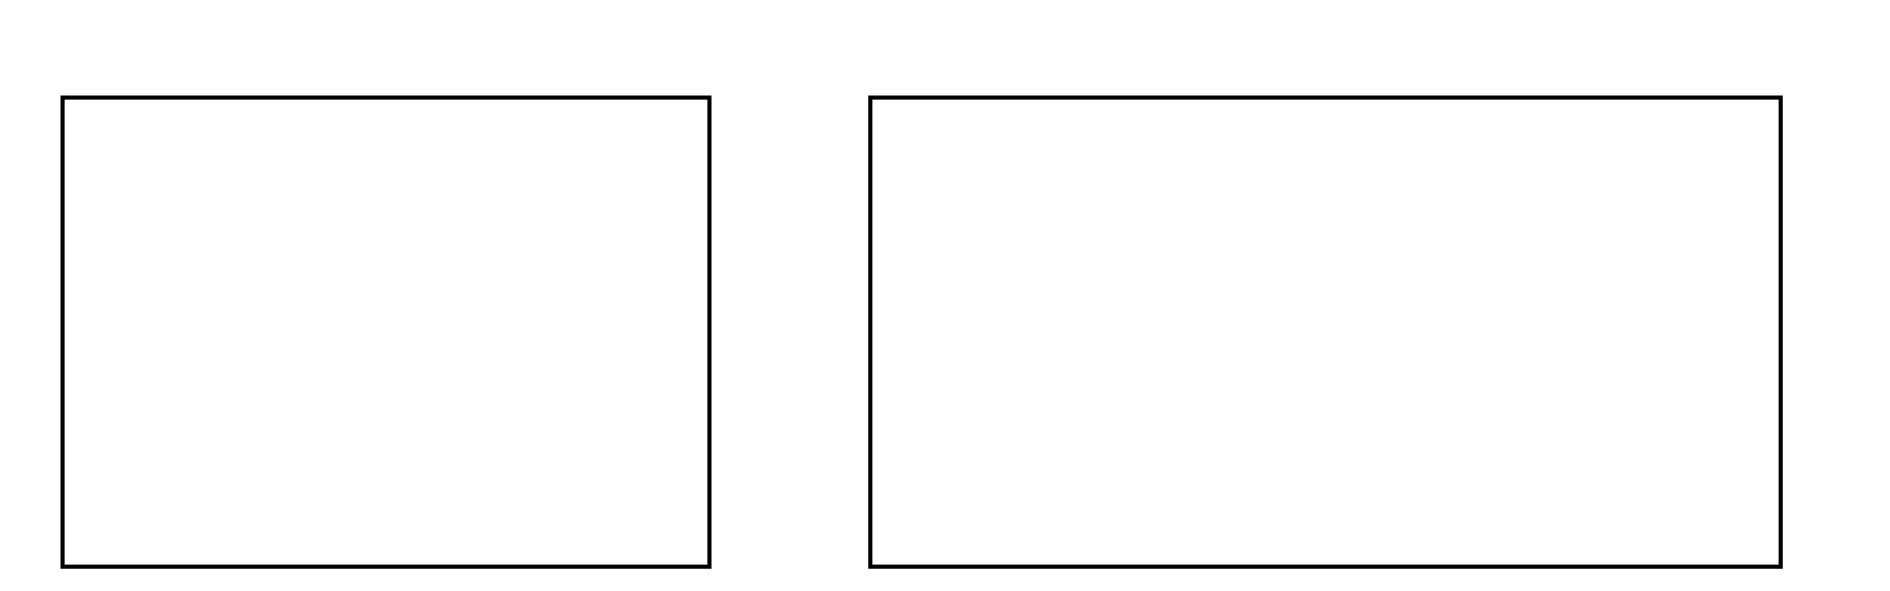
\includegraphics[width = 16cm]{Dissertation_char_vis_thg.jpg}
    \caption{Caption}
    \label{fig:mode_char_thg}
\end{figure}

Fitting the result with the Eq.~\ref{eq:thg_phase_mismatch} we determined the total loss as $\kappa_3 = 26$~MHz, which is comparable with the results obtained by the transmission technique. Using the same rate between the coupling and the intrinsic loss, we can estimate the values $\kappa_3^{(i)} = 8$~MHz and $\kappa_3^{(e)}=11$~MHz. 

An natural conclusion is think that is possible to use the Eq.~\ref{eq:out_wave} simultaneously with Eq.\ref{eq:thg_phase_mismatch} to, using a fit, determine the coupling rat; however, the fit would calculate the whole numerator, in other word, the fit determine the value of $\kappa_3^{(e)}|\omega_3 B_3 (a_1)^3|^2$, to use this information to infer the coupling rate we must first know the Coupling term $B_3$ and the infrared mode amplitude $a_1$, both aren't possible to directly measure which makes this procedure complicated and fragile due to errors propagation. 

In order to get a reliable estimate we must determine the Coupling term. As already seen, this term depends on the spatial distribution of the mode, which can't be measured but is calculated using simulation.

\section{Coupling Term Estimate}

The coupling terms $B_1$ and $B_3$ can't be directly measured. One way to estimate their values is be simulate the both modes, using Finite Element Method, to determine the spatial distribution and calculate the overlap integral, Eq.\ref{eq:overlap_j3}.

The simulation was made using the software COMSOL\regmark. Initially we calculate the dispersion of group of modes (10 modes for infrared and 100 for visible). We could calculate the Coupling Term between all of this modes, leading to a matrix if 10$\times$100 elements; however, most of the pair of modes can not coupling due to the phase matching condition. To filter we must assume that $3\times m_1 = m_3$. Also, we consider a finite linewidth for the mode. 

%There is a important subtlety when considered the phase matching to filter the modes. The linewidth showed in the transmission spectrum is a characteristic of the system 'cavity+taper' and not of the laser source, in fact the laser source is narrow enough to be considered single frequency when compared with the mode. The process is depicted in the Fig.. The photons of the laser (red line) confined in a infrared mode (dashed red line) will interact with the material of the cavity and will be scattered with exactly three times the frequency of the source creating the green line, which can be confined in a visible mode since it 


\section{THG Efficiency Mapping}
%Acho que não tem muito segredo nessa sessão. 
\chapter{Outlook}
% \begin{itemize}
%    \item Resultado do projeto
%    \item Contribuição do Projeto
%    \item Pontos que podem melhorar e previsões futuras
%\end{itemize}
%The results of the project can be summarized in technical advances and scientifical advances.

We have demonstrated generation of third harmonic in optical microcavities, with a maximum net efficiency of $10^{-5}$. 

The microcavities was fabricated using in-house facilities, which needed of a dedication in develop and describe the process of fabrication of wedge cavity. Even though the $Q$ factory of our cavities is some orders of magnitude lower than those already demonstrated in the literature, it was possible to identify the key problems which enable the group to precisely attack then, turn it spendless to solve. It was possible to describe the dynamics of the coupling of two modes due to third order nonlinearity. The numerical solution of the coupled rate equation showed a well qualitative agreement with the experimental result, and a satisfactory quantitative agreement, despite the limitation on determine the values  

The amount of visible light can by largely improve by increase the coupling between the source and the visible mode, the use of a different bus guide for the visible light was already demonstrated an efficient alternative~\needcit. The input power was a limitation to reach the maximum efficiency regime predicted in the model; however, a improvement in the $Q$ factor should decrease the critical power required enabling the study of the maximum regime efficiency. 
\appendix
\chapter{Appendex}
\label{app:Comsol_Solution}

\addcontentsline{toc}{chapter}{Referênciasbibliográficas}
\spacing{1.15}
{\footnotesize
%\bibliographystyle{unsrt_short}    %% numero
%\bibliography{relatorio_cpg}
}

\end{document}























    
    
    
    
    